\chapter{Implementation of Theory: What people and I did to implement the theory using computers}

Introduction: yadda yadda yadda (TODO)
\section{Methods}
\subsection{Rigorous Coupled Wave method: GSolver}
TODO

\begin{figure}[htbp] %  figure placement: here, top, bottom, or page
   \centering
   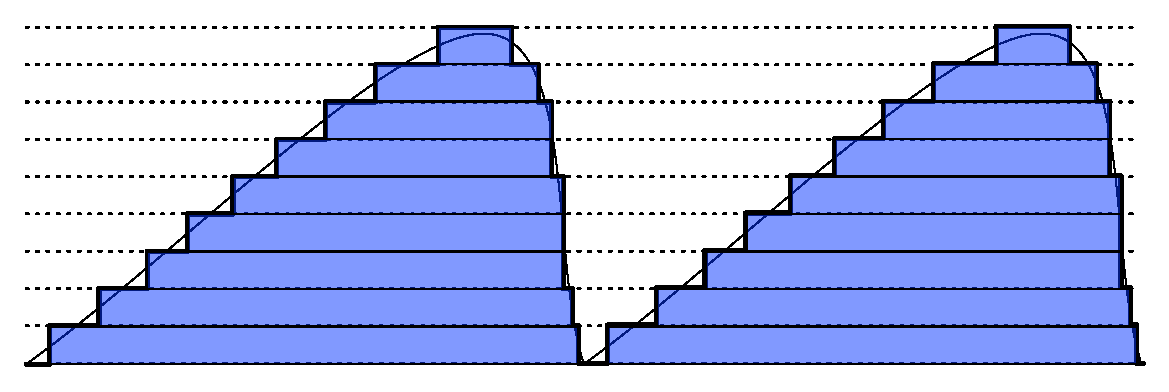
\includegraphics[scale=0.8]{Chapter3/3a_RCWA/3a.pdf} 
   \caption{The RCW method approximates every real grating as a stack of rectangular gratings, where the boundary conditions are easy to solve and the problem can be reduced to algebraic methods.}
   \label{3a}
\end{figure}

\subsection{Differential method: Gradif by Michel Neviere}
TODO


\section{Improving the usability and efficiency of calculation methods}
The Canadian Light Source purchased the Gradif code from Professor Neviere and made it available for this project.  However, there were two challenges involved in applying the code:
\begin{enumerate}
\item The code itself is an iteration on old Fortran program that provides no user interface.  Instead, to calculate an efficiency data point for a grating at just one energy, approximately 30 numbers must be entered into a blank screen, with no prompts, in the correct order.  These numbers define the grating geometry, the coating/layer thicknesses, the incidence conditions, the integration parameters, and also the complex refractive indices of the layers and the substrate.\footnote{These last two values will change as a function of photon energy, since the refractive index varies with wavelength, so we need to look them up for each data point.}  As a result, using this program requires a time-consuming and error-prone process.
\item In the event of an error made during the data entry process, one of many grating parameters could end up outside the narrow region of convergence where the code is able to  numerically integrate a solution successfully.  When this happens, the program runs forever in an infinite loop, with no feedback that the calculation has failed.  This region of convergence is not well established, so even when data entry errors are avoided, it's possible for a user to specify a valid grating that is -- for example -- too deep to be calculated.  Without user feedback, it's impossible to know if the calculation is still running successfully, or if it has failed into this infinite loop.
\end{enumerate}
To beat these two challenges, we built a web-based graphical interface, and carefully modified the Fortran source code to detect convergence failures.
\subsection{Visual interface to the Gradif code}
Figure \ref{3b} shows a screenshot of the graphical user interface (GUI) that we built to help us perform efficiency calculations quickly and efficiently.  The interface serves as a wrapper to generate input for the Gradif code, manages running a set of calculations, and extracts the results.

\begin{figure}[htbp] %  figure placement: here, top, bottom, or page
   \centering
   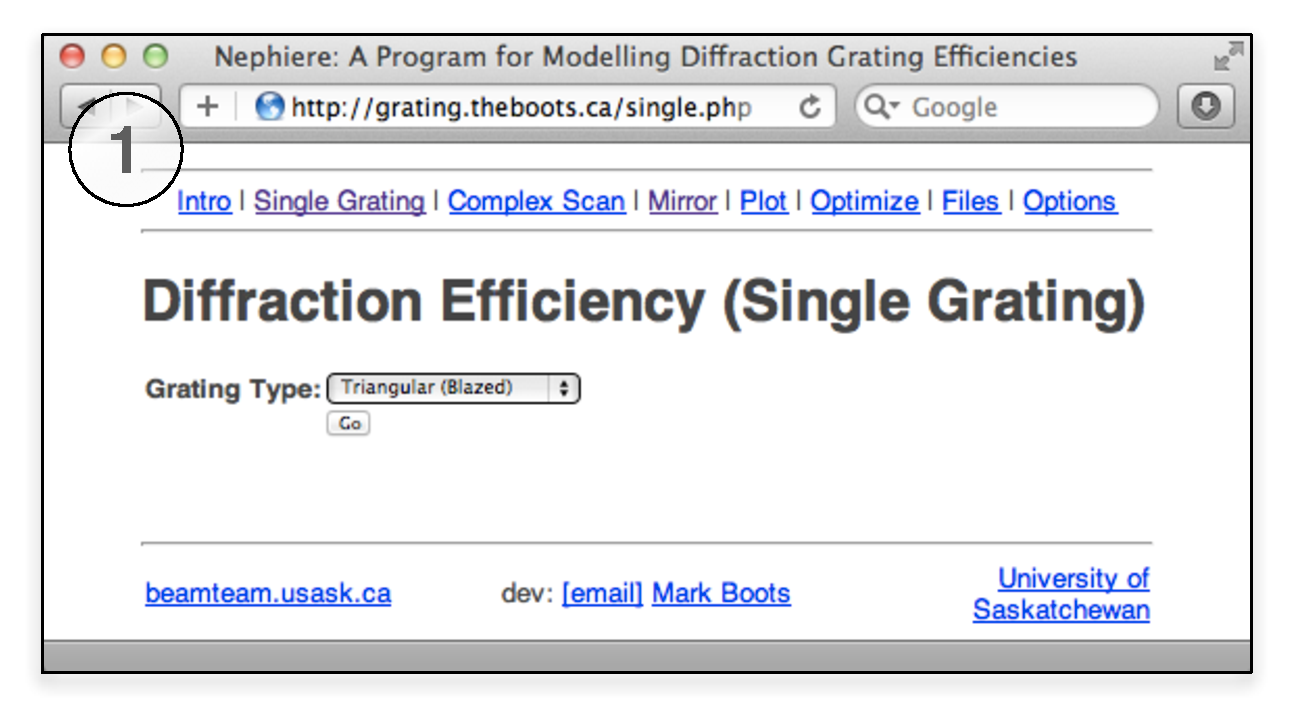
\includegraphics[scale=0.6]{Chapter3/3b_nephiere/3b_1.pdf} \\
%\vspace*{0.25in}
   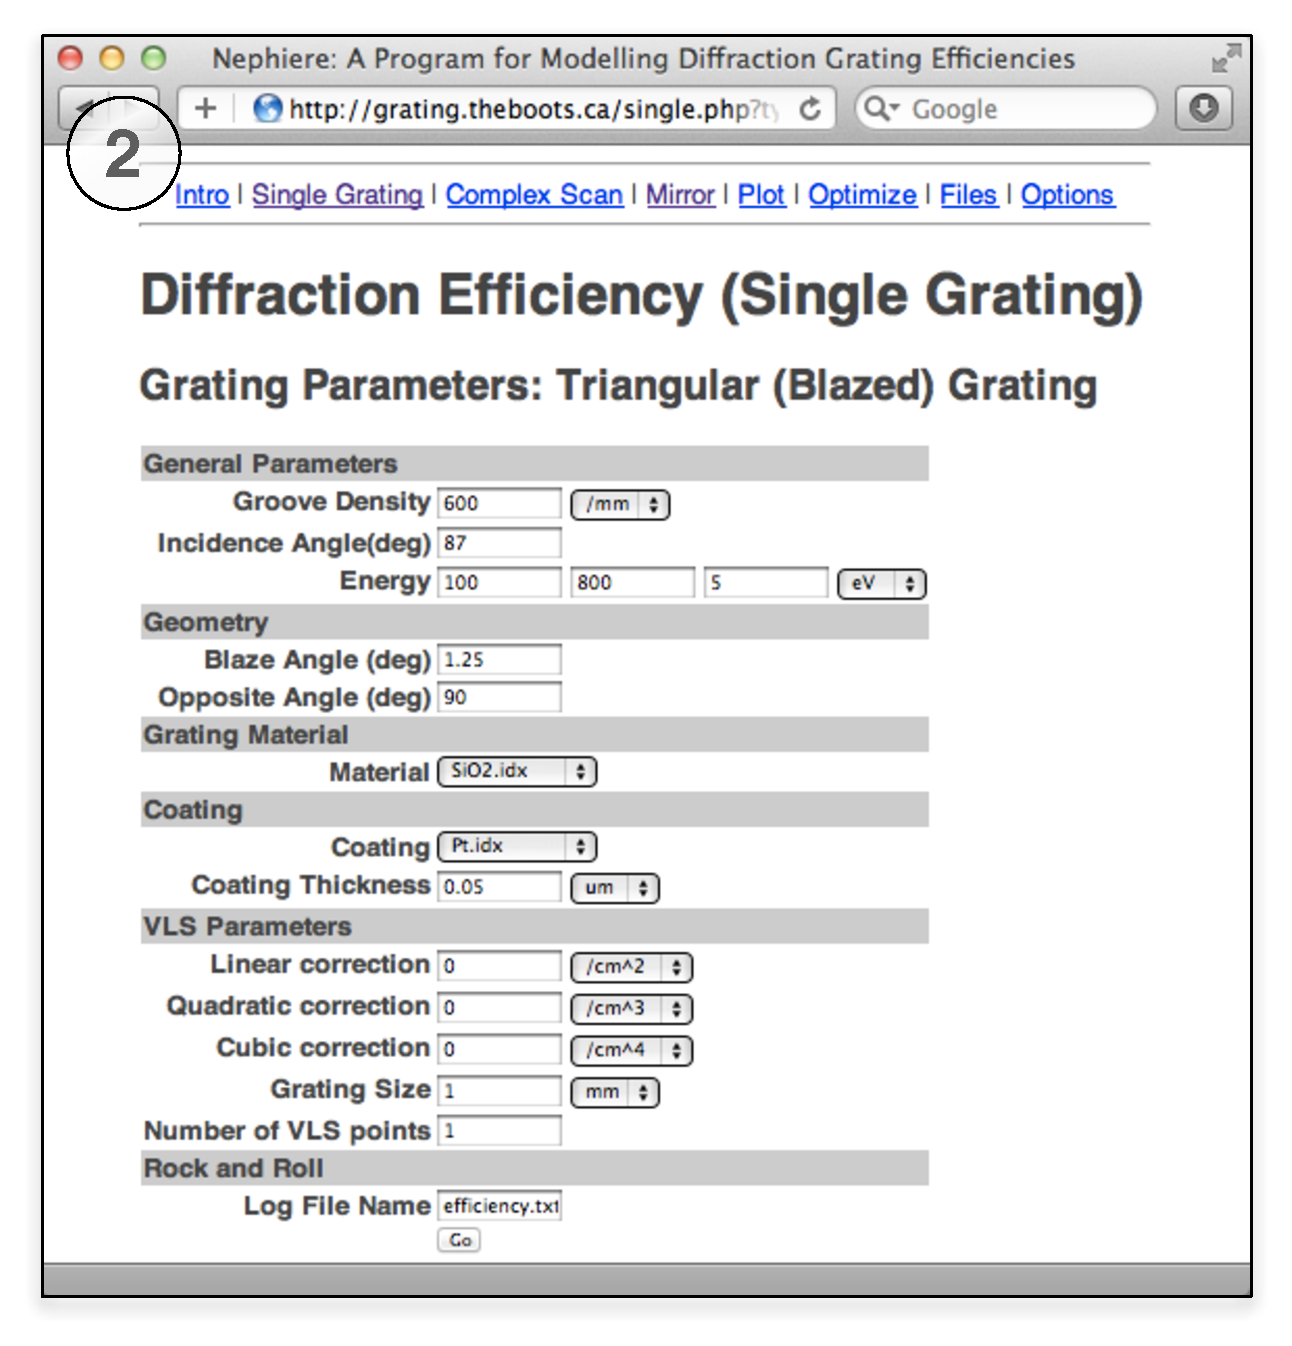
\includegraphics[scale=0.6]{Chapter3/3b_nephiere/3b_2.pdf}
   \caption{This web application provides a graphical user interface for calculating grating efficiencies. Forms prompt users for the grating parameters...}
   \label{3b}
\end{figure}

The interface was implemented as a web-based application, so it can be used from anywhere through a browser, without having to distribute the Gradif code or install anything on a person's individual computer.  Users describe the grating parameters and application scenario through a form that prompts them for the necessary information based on the type of grating (Figure \ref{3b}).  The results automatically generate a plot, and users can also download data tables of their calculations.  These tables are also archived so they can be retrieved later.

It supports the following features:
\begin{itemize}
\item \textbf{Grating Types}\\
The interface supports rectangular, blazed, trapezoidal, and sinusoidal grating profiles; it prompts for the geometry parameters that are required in each case.

\item \textbf{Order and Polarization}\\
Users can configure which inside and outside orders should be calculated, as well as specify the polarization of the incident light: TE, TM, or natural light (un-polarized).

\item \textbf{VLS Gratings}\\
To model variable line space gratings, the interface accepts the VLS parameters in conventional notation (linear, quadratic, and cubic corrections) and uses these to calculate the groove density and corresponding efficiency at a user-determined number of points along the grating surface; the overall efficiency is taken as an average of these.

\item \textbf{Efficiency plots as a function of wavelength}\\
The simplest way to use the interface generates a plot of the efficiency in the desired orders as a function of wavelength, holding all the other parameters constant (Figure \ref{3b_3}).  This is the most typical use-case for testing how a grating would perform in a beamline.

\begin{figure}[p] %  figure placement: here, top, bottom, or page
   \centering
   \vspace*{-.5in}
   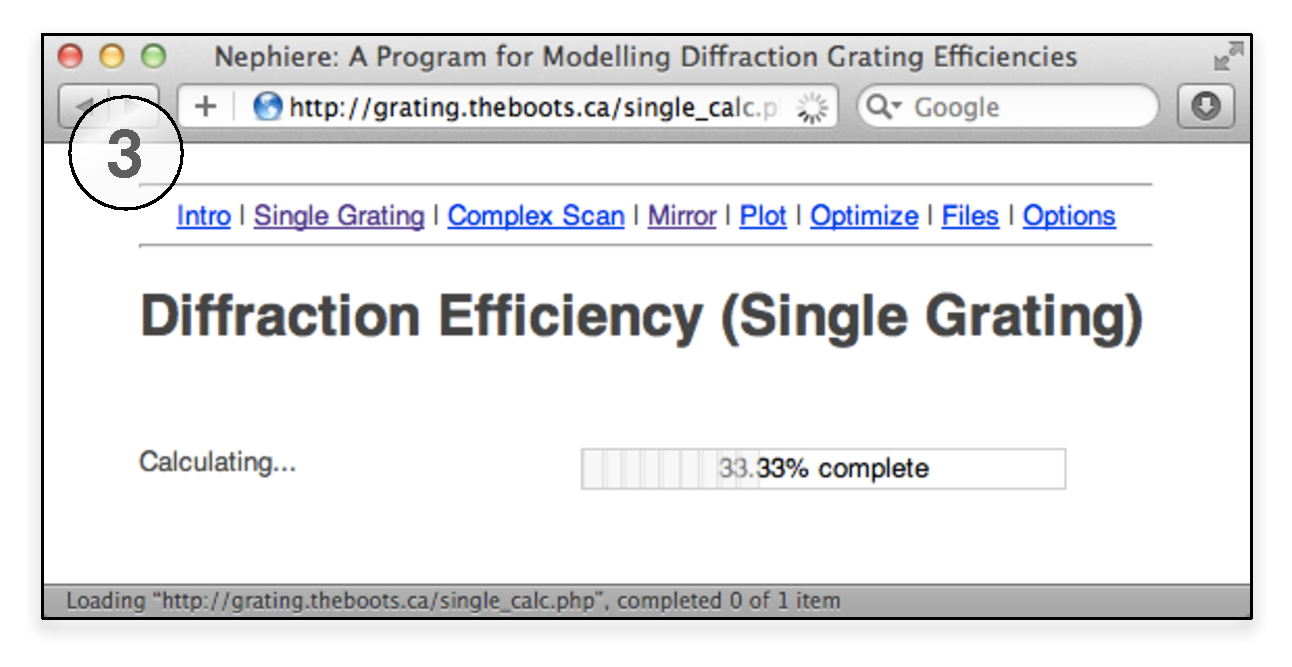
\includegraphics[scale=0.6]{Chapter3/3b_nephiere/3b_3.pdf} \\
%\vspace*{0.25in}
   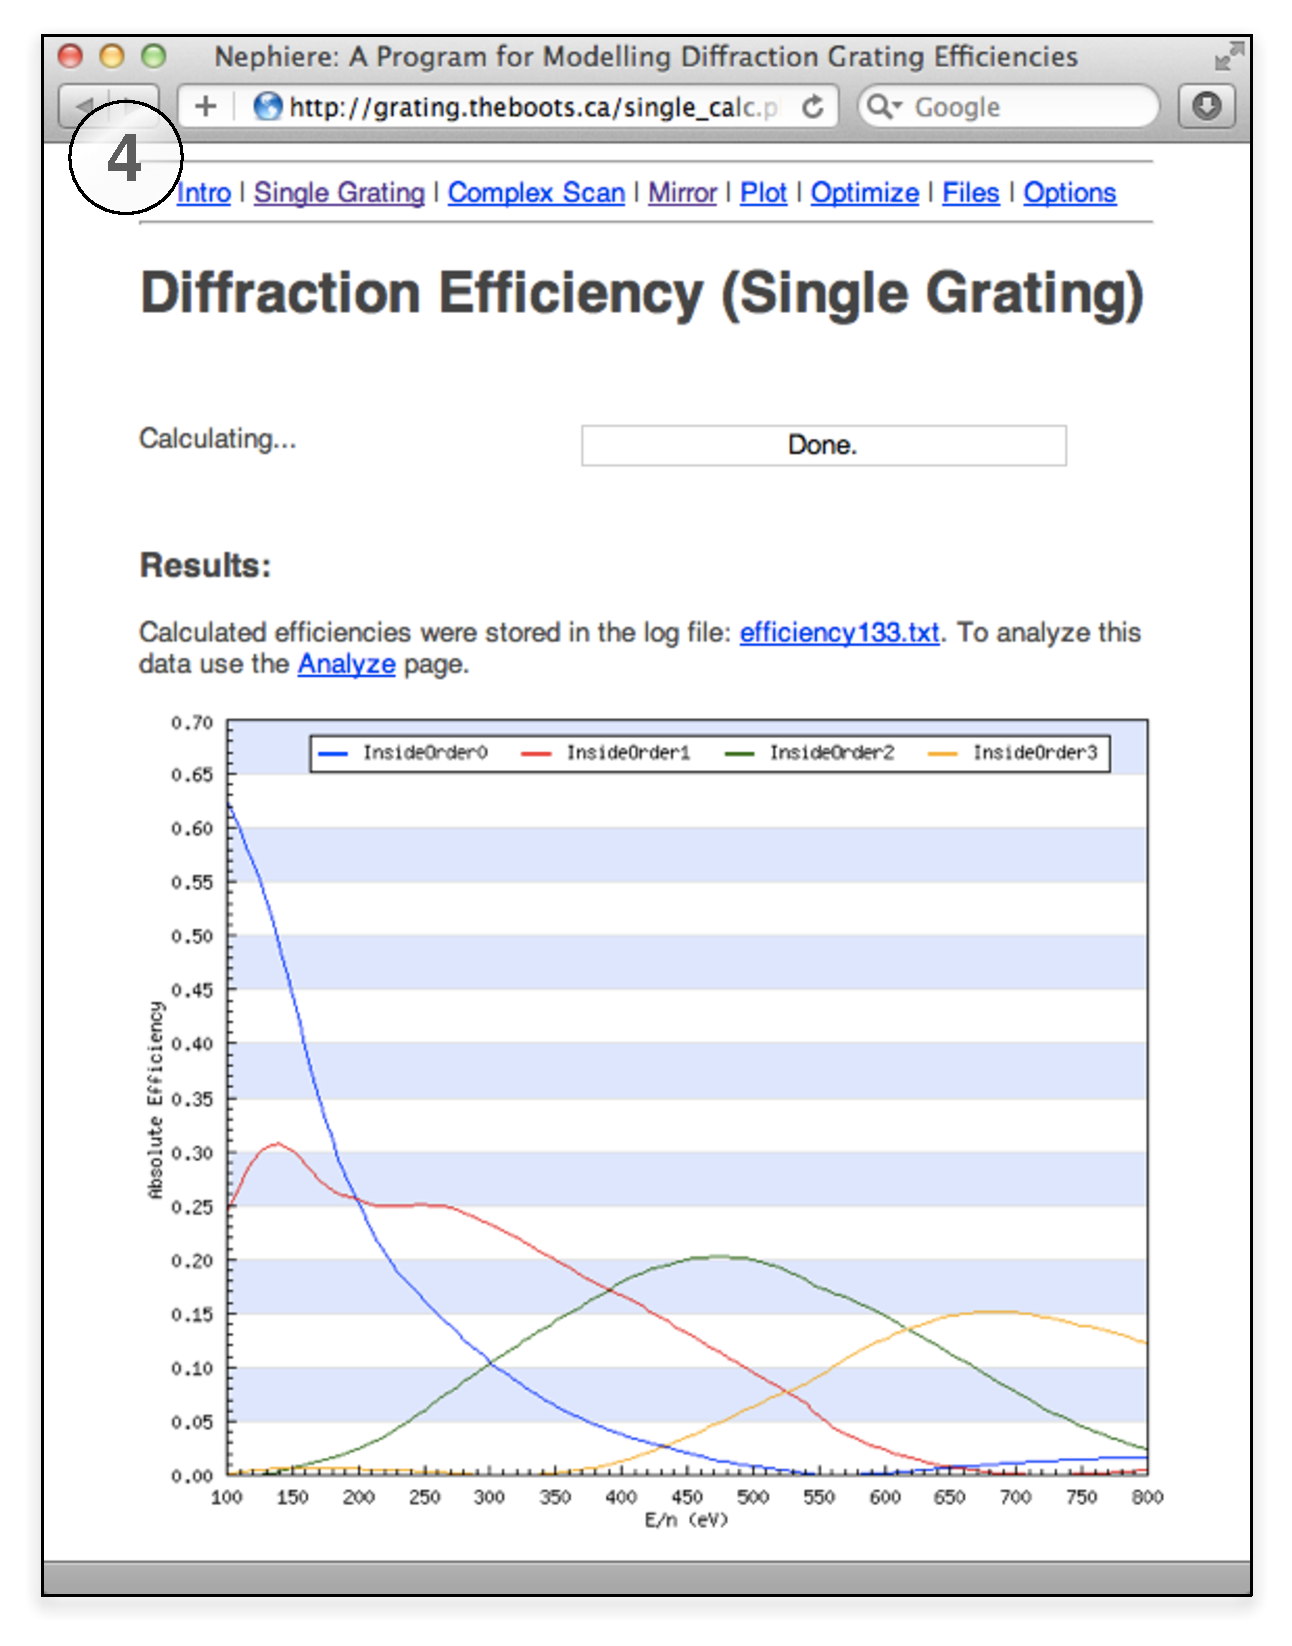
\includegraphics[scale=0.6]{Chapter3/3b_nephiere/3b_4.pdf}
   \caption{This web application provides a graphical user interface for calculating grating efficiencies. The results are plotted, and users can download a text-based table for further analysis.}
   \label{3b_3}
\end{figure}

\item \textbf{Complex scans over arbitrary grating parameters}\\
The interface also offers flexibility to test arbitrary relationships along incidence angle, energy, geometry, and other parameters. This feature is most efficiently used in conjunction with a spreadsheet or other data analysis program to fill in the grating parameters and interpret the data tables that are produced.

\item \textbf{Database of Optical Materials and Refractive Index}\\
We also developed a database of common grating substrate and coating materials, so that the interface can automatically look up their complex refractive index as a function of photon energy.  This information was calculated using the semi-empirical Henke data tables of the x-ray atomic form factor (TODO ref).  The current library is valid from 30eV to 10~000eV, but is known to have limited accuracy in the immediate neighborhood of absorption edges.

\item \textbf{Mirror Reflectivity}\\
As an additional tool for beamline designers, we implemented the ability to calculate the reflectivity of a simple mirror using any of the materials in the refractive index database.  Mirror reflectivities are computed as a function of incidence angle and photon energy using the complex Fresnel equations (TODO ref Modern Optics), and are subject to the same options for polarization.

\item \textbf{Control of Numerical Precision}\\
An `Options' page (Figure \ref{3b_5}) allows users to configure the numerical precision used in the calculations.  The two critical factors are the number of integration steps used in the numerical integration of the particular solutions for the $A_n^{(m)}$ and $B_n^{(m)}$ coefficients at each layer, and the number of Fourier coefficients $N$ used before the sum is truncated.  The defaults we chose ($N=31$; 401 integration steps) have been found to produce accurate results reasonably quickly across the entire soft x-ray range, as long as the coating thickness is less than 0.5um.   However, prudent designers should still do convergence tests for any high-stakes results, by repeating the calculations and comparing against efficiencies computed using larger values.  This technique can also be used to find the minimum number of Fourier coefficients that are required before the results start to disagree.  (This can helpful to optimize the computation speed before running a large number of calculations on similar gratings at similar wavelengths.)
\end{itemize}

\begin{figure}[p] %  figure placement: here, top, bottom, or page
   \centering
   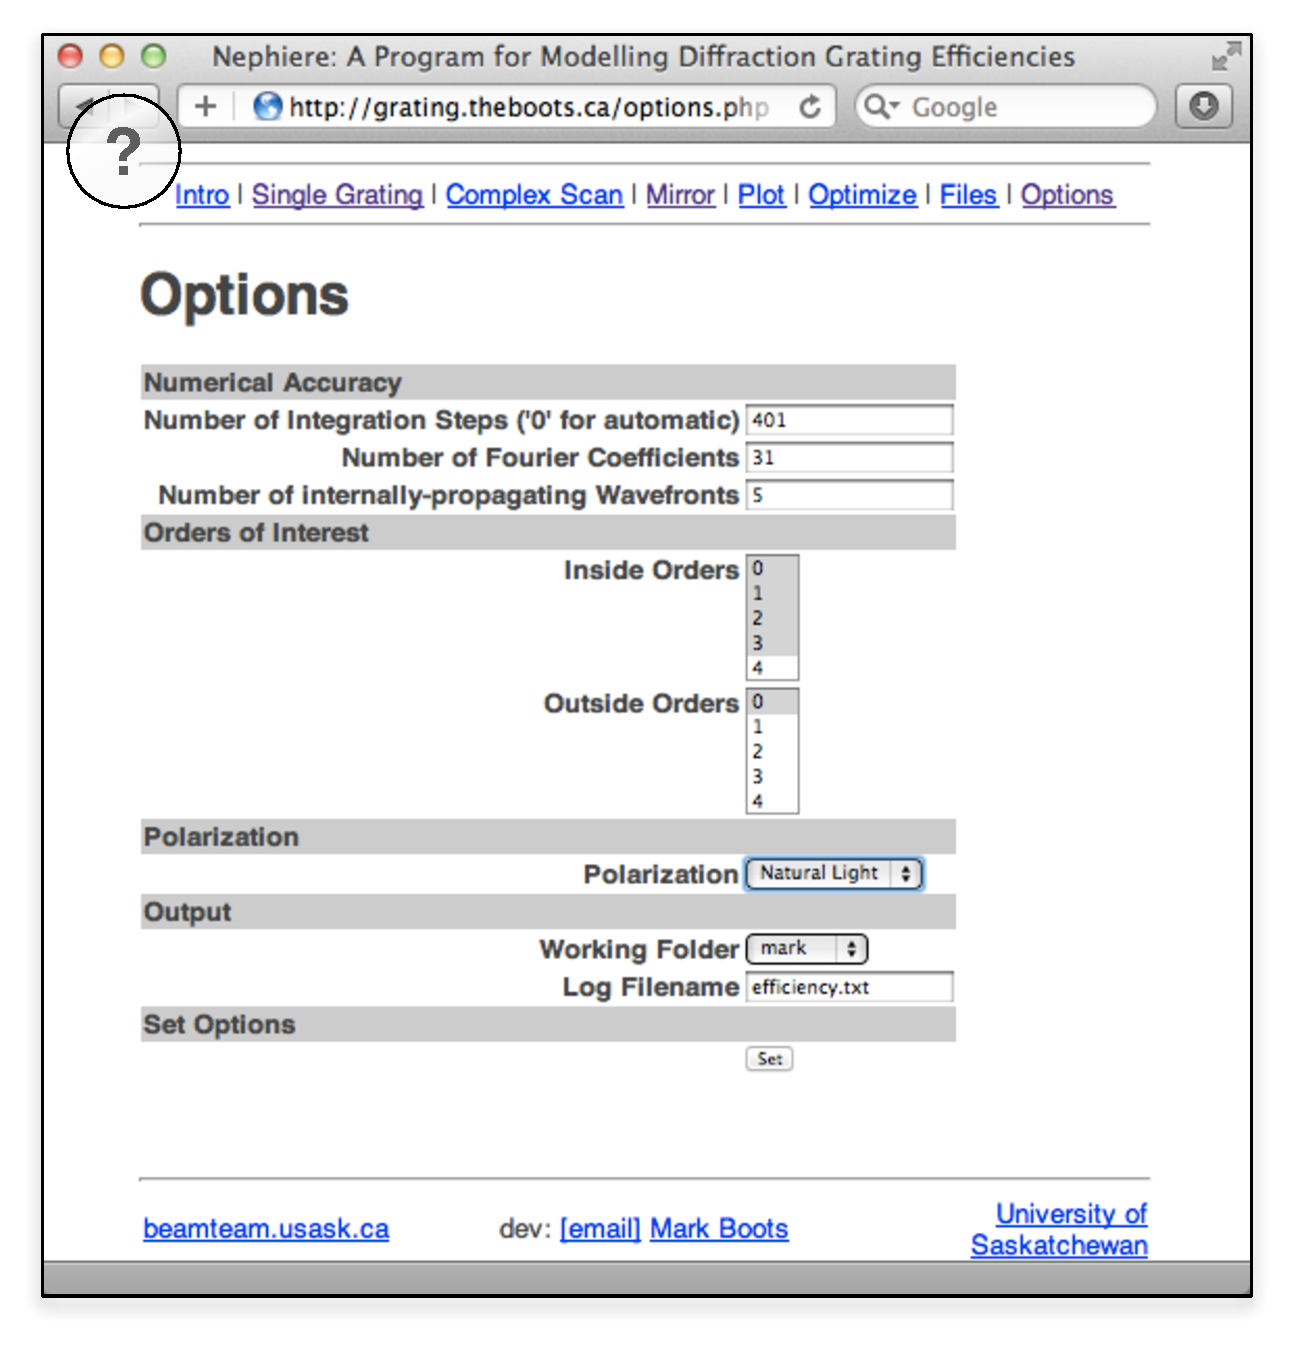
\includegraphics[scale=0.6]{Chapter3/3b_nephiere/3b_5.pdf}
   \caption{This `Options' page configures the numerical precision of the calculations, the diffraction orders of interest, and the polarization of the incident light.  It also sets some other house-keeping options for where users want to store their data.}
   \label{3b_5}
\end{figure}

\subsection{Detecting convergence failures}
The Fortran code that makes up the Gradif program was written using a 1970's-era programming approach, including prodigious use of global variables and GOTO statements.  (These two features are now heavily discouraged in modern programming methedologies.)  As a result, the code is hard to trace, but we were able to insert a counter to detect when a numerical integration fails to converge after multiple attempts.  This allows the calculation to exit with an error message, rather than run indefinitely.

\subsection{Open Source, Open Access, and Future Work}
Since we released the user interface under an `open-source' license, it can be upgraded or enhanced by anyone with an interest in the beamline design community.  Julian Miller, a summer student in the metrology department at the CLS, recently created an updated version of the interface to support multi-threaded calculations and add more options for incidence configurations.  To the original `constant incidence angle' mode, he added a `constant included angle' mode, used in many monochromators, which tilts the grating as a function of photon energy to maintain a constant angle between the incident and outgoing beam in the desired order.  Since every grating efficiency calculation (at a single energy) is independent, they can be run in parallel; this takes advantage of modern multi-core processors, and dramatically speeds up the creation of a user's plot or data set.  In the future, this could be extended even further to spread calculations over a cluster of computers, or on distributed hardware in a `cloud computing' network.

Because the user interface runs as a web application, it can be (and has been) accessed by beamline designers from all over the world.  As one example, it was used by Professor Coryn Hague to improve the design of a new beamline for the SOLEIL synchrotron (TODO find ref).  The calculations can be requested and retrieved by anyone from anywhere, but they all run on a single server computer at the University of Saskatchewan.  Unfortunately, the Gradif code itself is not open source, and while we are licensed to run it on this machine, recent communications from Professor Neviere indicate that he is unhappy with this level of open access to results produced using his Gradif engine.  As a result, we have temporarily disabled public access.

In the future, we plan to completely re-implement the core engine for calculating efficiencies, according to the theory outlined in this thesis.  This will allow us to optimize the the computation speed by employing per-calculation multi-threading and a modern high-performance programming language.  This will also allow us to distribute a completely open version of the whole system, un-encumbered by licensing issues.  Finally, we plan to combine this with Julian's work and other upgrades to the usability of the web interface.

\section{General trends and factors affecting efficiency}
With these tools in-hand, we move on to the next question: What can we learn from them about the efficiency of gratings, especially those used in the soft x-ray regime?

This section looks at the theoretical effects caused by changes to grating parameters: groove profile, shape (depth, duty cycle, blaze angle, etc.), line density, coating material, coating thickness, and incidence angle.  We can think of the grating efficiency as a scalar function of this many-dimensional parameter space, but it's impossible to capture its complexity in a simple analytical equation.  None the less, the results of this section should give beamline designers an understanding of trends along each dimensions within this space, and how to apply these trends to the optimization of gratings.

We attempt to isolate the effects of each parameter as much as possible.  However, many parameters are linked together so that they cannot be made independent.  For example, as we show in Section \ref{blazeAngle}, gratings with triangular profiles have an optimal \emph{blaze angle} which aligns the outgoing diffraction order with the specular reflection for maximum efficiency.  For this type of grating, changing only the groove density will change the outgoing diffraction angle, and therefore change the optimal blaze angle.  Simply plotting the efficiency as a function of groove density while holding all other parameters constant would confuse the blaze effect with the density effect; instead, we correct for this by adjusting the angle to keep the grating ``on-blaze'' as we vary the groove density in Figure \ref{3e}.

\subsection{Effect of Grating Profile: Groove Shape}

As we showed in Chapter 3, any kind of periodic groove structure will have a diffraction effect, regardless of the nature of the groove shape.  However, the grating efficiency -- particularly in the order the experimenter wants to usue -- depends substantially on the groove shape.  

Five common groove profiles are shown in Figure \ref{3c-profile}: a classic rectangular profile, a triangular profile (also known as a ``sawtooth'' or ``blazed'' pattern), a trapezoidal profile, a sinusoidal profile, and an approximated triangular profile.

\begin{figure}[htbp] %  figure placement: here, top, bottom, or page
   \centering
   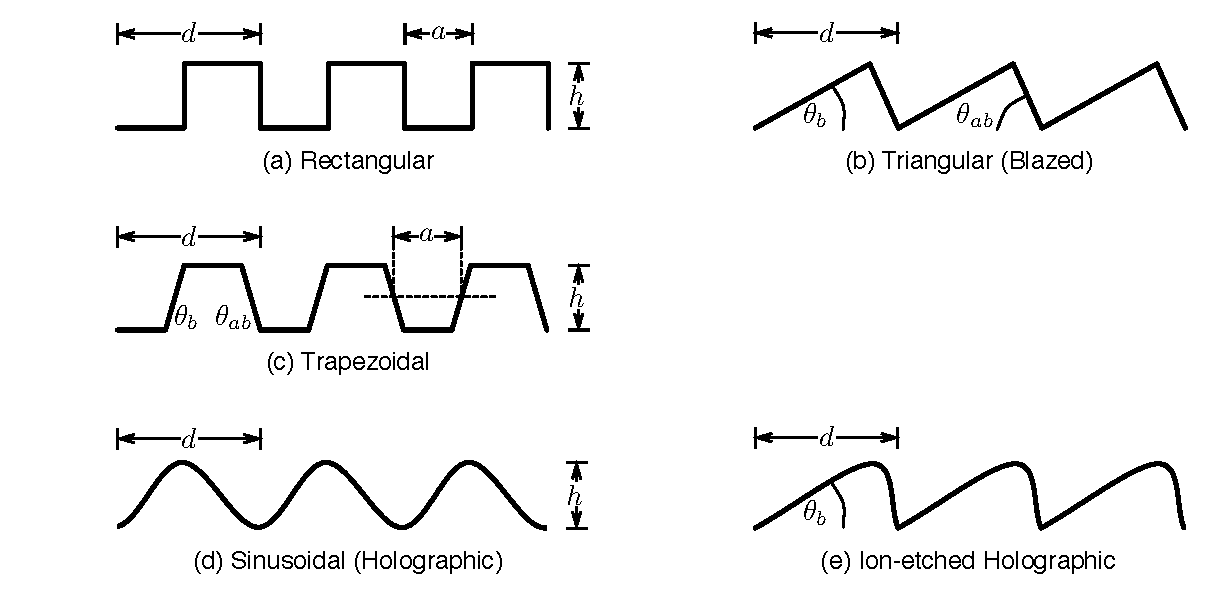
\includegraphics[scale=0.8]{Chapter3/3c_effectOfProfile/3c_profiles.pdf}
   \caption{5 common groove profiles and their geometry parameters.  The rectangular profile (a) and triangular profile (b) are idealized versions of those produced by mechanical ruling.  The trapezoidal profile (c) is usually produced accidentally while trying to rule a rectangular profile with an imperfect ruling tip.  The sinusoidal profile (d) is the natural shape produced by holographic ruling; the result can be ion-etched to approximate a triangular profile (e).}
   \label{3c-profile}
\end{figure}

\subsubsection{Grating Manufacturing Techniques}
These types of profiles emerged largely as a consequence of grating manufacturing techniques.  Henry Rowland invented a method for machining long, precise screws (TODO ref), and this enabled him to create a ``ruling engine'' (Figure \ref{3c-rowlandEngine}) for mechanically scratching fine parallel lines into a layer of metal on a substrate material.  His version was much more accurate than previous machines because it self-compensated for systematic errors in the screw pitch, and his efficient production of high-quality gratings ``revolutionized spectroscopy'' (TODO http://www.aip.org/history/gap/Rowland/Rowland.html).  Today, there are several extremely precise ruling engines around the world, using diamond tips and interferometric position feedback to mechanically engrave groove densities approaching 3~000 lines/mm.\footnote{The Michelson ruling engine at the Newport Corporation can rule up to an astonishing 10~800 lines/mm.}

The rectangular and triangular profiles in Figure \ref{3c-profile} are a consequence of the shape of mechanical ruling tips.  The trapezoidal profile is often produced accidentally when attempting to rule a rectangular profile with a non-ideal tip, as was the case for the gratings shown in Figures \ref{3j-3} and \ref{3j-4}.

\begin{figure}[htbp] %  figure placement: here, top, bottom, or page
   \centering
   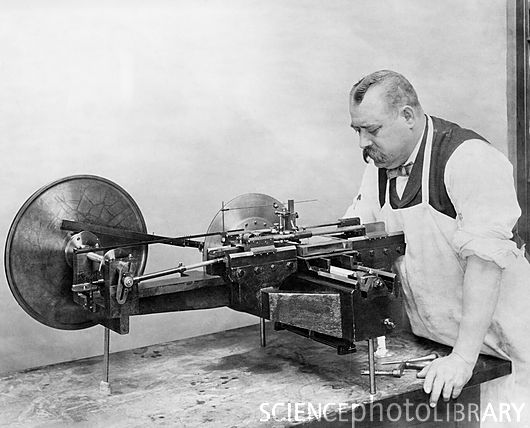
\includegraphics[width=0.8\textwidth]{Chapter3/3c_effectOfProfile/rowlandRulingEngine.jpg}
   \caption{Henry Rowland's ruling engine, mechanically engraving a grating under the operation of his instrument maker Theodore Schneider.  Photographed at Johns Hopkins University, Baltimore.  \textbf{Image credit: }\textsc{Emilio Segre Visual Archives/American Institute Of Physics/Science Photo Library} (TODO ref http://www.sciencephoto.com/media/150151/enlarge)}
   \label{3c-rowlandEngine}
\end{figure}

\begin{figure}[htbp] %  figure placement: here, top, bottom, or page
   \centering
   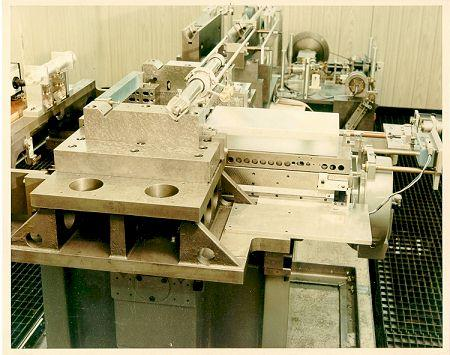
\includegraphics[width=0.8\textwidth]{Chapter3/3c_effectOfProfile/mitBRulingEngine.jpg}
   \caption{The MIT `B' ruling engine, now owned and operated by Richardson Gratings (a division of the Newport Corporation).  It can rule gratings up to 420 mm wide, with grooves up to 320 mm long.  The maximum groove density is 1500 lines/mm.  Equipped with a servo system for advancing the grating carriage and interferometric feedback using frequency-stabilized lasers, it is the most accurate ruling engine in the world.  To control for thermal expansion of the engine, the room temperature is controlled to 0.005$\deg$C; the system even compensates for changes in room air pressure since a change of just 2.5 mm of mercury will affect the refractive index of air (and therefore the interferometer wavelength) by one part per million.  The entire engine is suspended from springs to dampen vibrations between 3Hz to 60Hz, which could otherwise be transmitted to the diamond tip.  \textbf{Image credit: }\textsc{Diffraction Grating Handbook} (TODO REF).}
   \label{3c-mitBEngine}
\end{figure}

The setup and operation of mechanical ruling engines is a long, elite, and painstaking process; for gory details, see (TODO REF http://gratings.newport.com/information/handbook/chapter3.asp) by the Newport Corporation, which operates three ruling engines.  To reduce the cost of ruled gratings, often a ``master grating'' is ruled mechanically and then used to create a mould for replicating other gratings; the groove shape is transferred using a thin layer of liquid resin which is hardened while in contact with the master grating surface (Figure \ref{3c-replication}).\footnote{The gratings used for the REIXS spectrometer were all master gratings. They were ruled directly into a smooth gold coating on top of a quartz grating blank, and then top-coated with an evaporated platinum or nickel surface.}

\begin{figure}[htbp] %  figure placement: here, top, bottom, or page
   \centering
   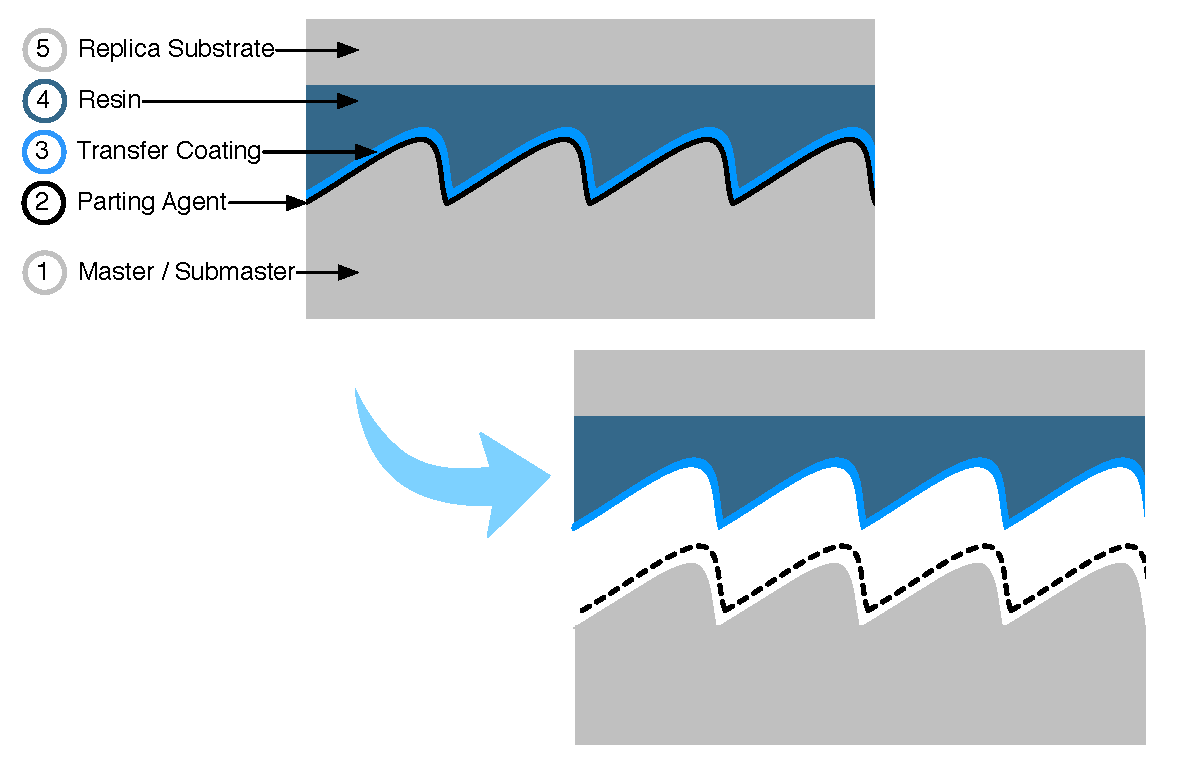
\includegraphics[scale=0.8]{Chapter3/3c_effectOfProfile/3c_replica.pdf}
   \caption{Master gratings can be replicated using a resin which hardens while in contact with the master (or subsequently, a submaster replicated from the first master).  First, a parting agent (2) is applied to the surface of the master; it must be thin and uniform otherwise it will affect the profile.  A metallic (aluminum or gold) coating about 1um thick is then applied above the parting agent; this coating will eventually end up as the top surface of the replicated grating, and is called the \emph{transfer coating} (3).  Finally, the replica blank (5) is cemented from above using a resin ($\sim$10um thick) that hardens under UV exposure or over time (4).  Once the resin is cured, the gratings are separated at the parting agent layer, leaving the hardened resin in the shape of the grooves, with the metal coating adhered to the top.  This will produce a mirror image of the master grating; to create a perfect replica, this first replica needs to be replicated again.  \textbf{Image credit: }\textsc{Diffraction Grating Handbook} (TODO REF).}
   \label{3c-replication}
\end{figure}

A more recent technique was invented in the late 1960s for manufacturing gratings faster and with more repeatability.  It uses two sources of coherent light to project a  holographic interference pattern of regular standing waves onto a grating master.  The grating master consists of a photoresist material that is either strengthened or weakened by exposure to light.  After the master has been exposed to the interference pattern for a sufficient time, it is bathed in a developer chemical, which washes away either the exposed or unexposed parts, leaving behind a sinusoidal relief pattern that corresponds to the original intensity of light (TODO REF  S. Lindau, "The groove profile formation of holographic gratings," Opt. Acta 29, 1371-1381 (1982).).

The last groove profile shown in Figure TODO represents an attempt to turn holographically-ruled sinusoidal gratings into triangular gratings using ion etching to partially eat away the groove surface while holding the finished photoresist master at an angle to the ion beam (TODO REF http://www.tandfonline.com/doi/abs/10.1080/713819374).  Another technique for pseudo-blazed holographic gratings is known as Sheridon's Method (TODO REF N. K. Sheridon, "Production of blazed holograms," Appl. Phys. Lett. 12, 316-318 (1968).), which uses a transparent photoresist, exposed to the intersection of a coherent light source with its reflected self (Figure \ref{3c-sheridon}).  Because the master is inclined relative to the interference pattern, the intensity profile is asymmetric and produces a lopsided sinusoidal shape.

\begin{figure}[htbp] %  figure placement: here, top, bottom, or page
   \centering
   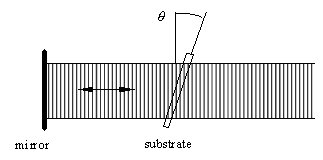
\includegraphics[scale=1]{Chapter3/3c_effectOfProfile/sheridonRecordingMethod.png}
   \caption{The Sheridon technique for recording pseudo-blazed holographic gratings uses a single light beam reflected back on itself to make a regular interference pattern of standing waves.  The master substrate consists of a \emph{transparent} photoresist material which is hardened or weakened by exposure to the light.  By placing the substrate at an angle $\theta$ to the light path, the light and dark fringes are stretched out parallel to the grating surface; additionally, the angled incidence creates a lopsided sinusoidal intensity pattern that mimics blazed gratings. \textbf{Image credit: }\textsc{Diffraction Grating Handbook} (TODO REF).}
   \label{3c-sheridon}
\end{figure}


\subsubsection{Profile Geometry}
Figure \ref{3c-profile} shows the parameters that describes that describe the geometry of each profile.  In addition to the groove spacing $d$, rectangular gratings are characterized by a groove depth $h$ (or duty cycle) and a groove width $a$.  Ruled triangular gratings are described by their blaze angle $\theta_b$; ideally the opposite angle (or ``anti-blaze angle'' $\theta_{ab}$) would be 90$\deg$ but often it ends up closer to 60$\deg$ or even 30$\deg$.  Trapezoidal gratings are described by a groove depth $h$, a groove width $a$, and their blaze and anti-blaze angles $\theta_b$ and $\theta_{ab}$.  Sinusoidal gratings are fully described by just their groove depth $h$, and an assumption of a sinusoidal variation $y(x) = y_0 + \frac{h}{2}\, \sin(2\pi \,x / d)$.

\subsubsection{Blazed Optimization for Triangular Gratings}
\label{blazeAngle}
The triangular profile in Figure \ref{3c-profile} (b) is much more than an accidental artifact of mechanical ruling.  This shape is optimal for concentrating as much energy as possible into a single order, and therefore boosting the grating efficiency in that order.  Intuitively, we might imagine that to increase efficiency, we should line up the direction of classical ``reflection'' off the majority of the grating surface with the direction of the diffracted ray.  Still thinking classically, we might also want to minimize shadowing in the corners of the grooves. 

The ideal blazed grating meets both of these criteria.  By carefully choosing a blaze angle $\theta_b$ we can -- at least at one wavelength of interest -- line up the specular reflection of the angled surface with the diffraction direction in order $n$.  Using the law of reflection from geometric optics ($\theta_{\mathrm{incident}} = \theta_{\mathrm{reflected}}$), we can easily\footnote{Setting up a ruling engine to correctly and accurately engrave this angle is another story...} derive the optimized condition for a blazed grating.  From the geometry in Figure \ref{3d}, where $N^\prime$ is normal to the angled surface: 
\begin{eqnarray}
\theta_{\mathrm{incident}} &=& \theta_{\mathrm{reflected}} \\
\theta_2 - \theta_b &=& \theta_{2,n} + \theta_b \\
\theta_{2,n} - \theta_{2} &=& -2 \theta_b
\end{eqnarray}
Applying a trigonometric identity to the grating equation (\ref{gratingEquation}):
\begin{eqnarray}
n\lambda / d &=& \sin\theta_{2,n} - \sin\theta_{2} \\
\frac{n\lambda}{2d} &=& \cos \left( \frac{\theta_{2,n} + \theta_{2}}{2} \right) \sin \left( \frac{\theta_{2,n} - \theta_{2}}{2} \right) \\
\frac{n\lambda}{2d} &=& \cos \left( \frac{\theta_{2,n} + \theta_{2}}{2} \right) \sin \left( -\theta_b \right) \\
\end{eqnarray}
or
\begin{eqnarray}
\label{blazeAngleEqn}
\theta_b = -\arcsin \left(   \frac{n \lambda}{2d \, \cos \left( \frac{\theta_{2,n} + \theta_{2}}{2} \right)}     \right)
\end{eqnarray}

\begin{figure}[htbp] %  figure placement: here, top, bottom, or page
   \centering
   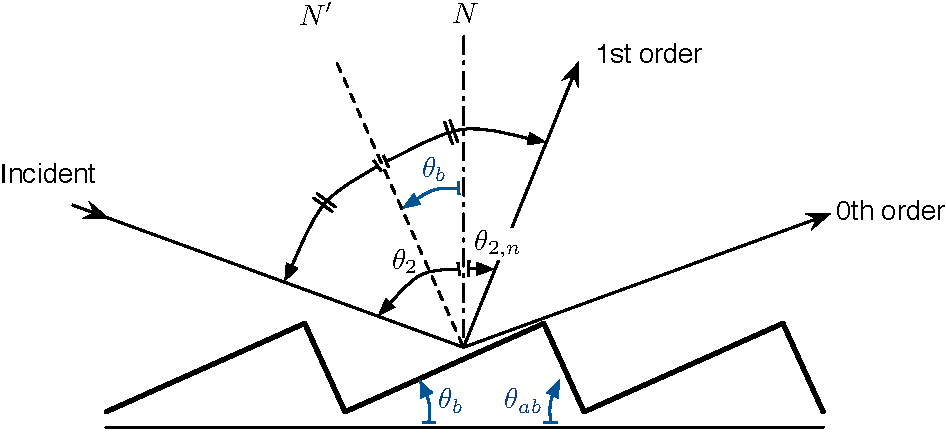
\includegraphics[scale=1]{Chapter3/3d_blazing/3d.pdf} 
   \caption{In the blazed condition, the desired order diffraction angle -- in this case, 1st order -- is aligned with the direction of specular reflection off the groove surfaces.}
   \label{3d}
\end{figure}

Textbooks and resources on beamline design universally provide this derivation and formula for the optimal blaze angle $\theta_b$ (TODO ref: CXRO x-ray data book, diffraction grating handbook, gratings slits and mirrors).  Using efficiency calculations, we've confirmed that this intuitive argument is a very good approximation for what happens in the full electromagnetic picture; the actual ideal blaze angle is usually slightly but insignificantly lower.  For a 1200 line/mm grating used at an incidence angle of 88 degrees with 400eV photons in the first inside order ($n=-1$) (Figure \ref{3c}), Equation \ref{blazeAngleEqn} would recommend a blaze angle of 1.67$\deg$.  We used this as the starting point to conduct a software optimization using efficiency calculations, and were only able to increase the 1st order efficiency from 16.2\% to 16.8\% by reducing the blaze angle from 1.67$\deg$ to the optimal 1.46$\deg$.

Because the blaze angle depends on the $n \lambda$ term in the grating equation, a grating optimized for a wavelength $x$ in 1st order will also be optimized for a wavelength $x/2$ in 2nd order (or, in terms of energy, optimization for $x$ eV in 1st order would imply optimization for $2x$ eV in 2nd order).  We can confirm this for the blazed grating in Figure \ref{3c-plot}, where the 1st-order efficiency peak occurs at 450eV, and the 2nd order efficiency peak occurs near 900eV.

\begin{figure}[htbp] %  figure placement: here, top, bottom, or page
   \centering
   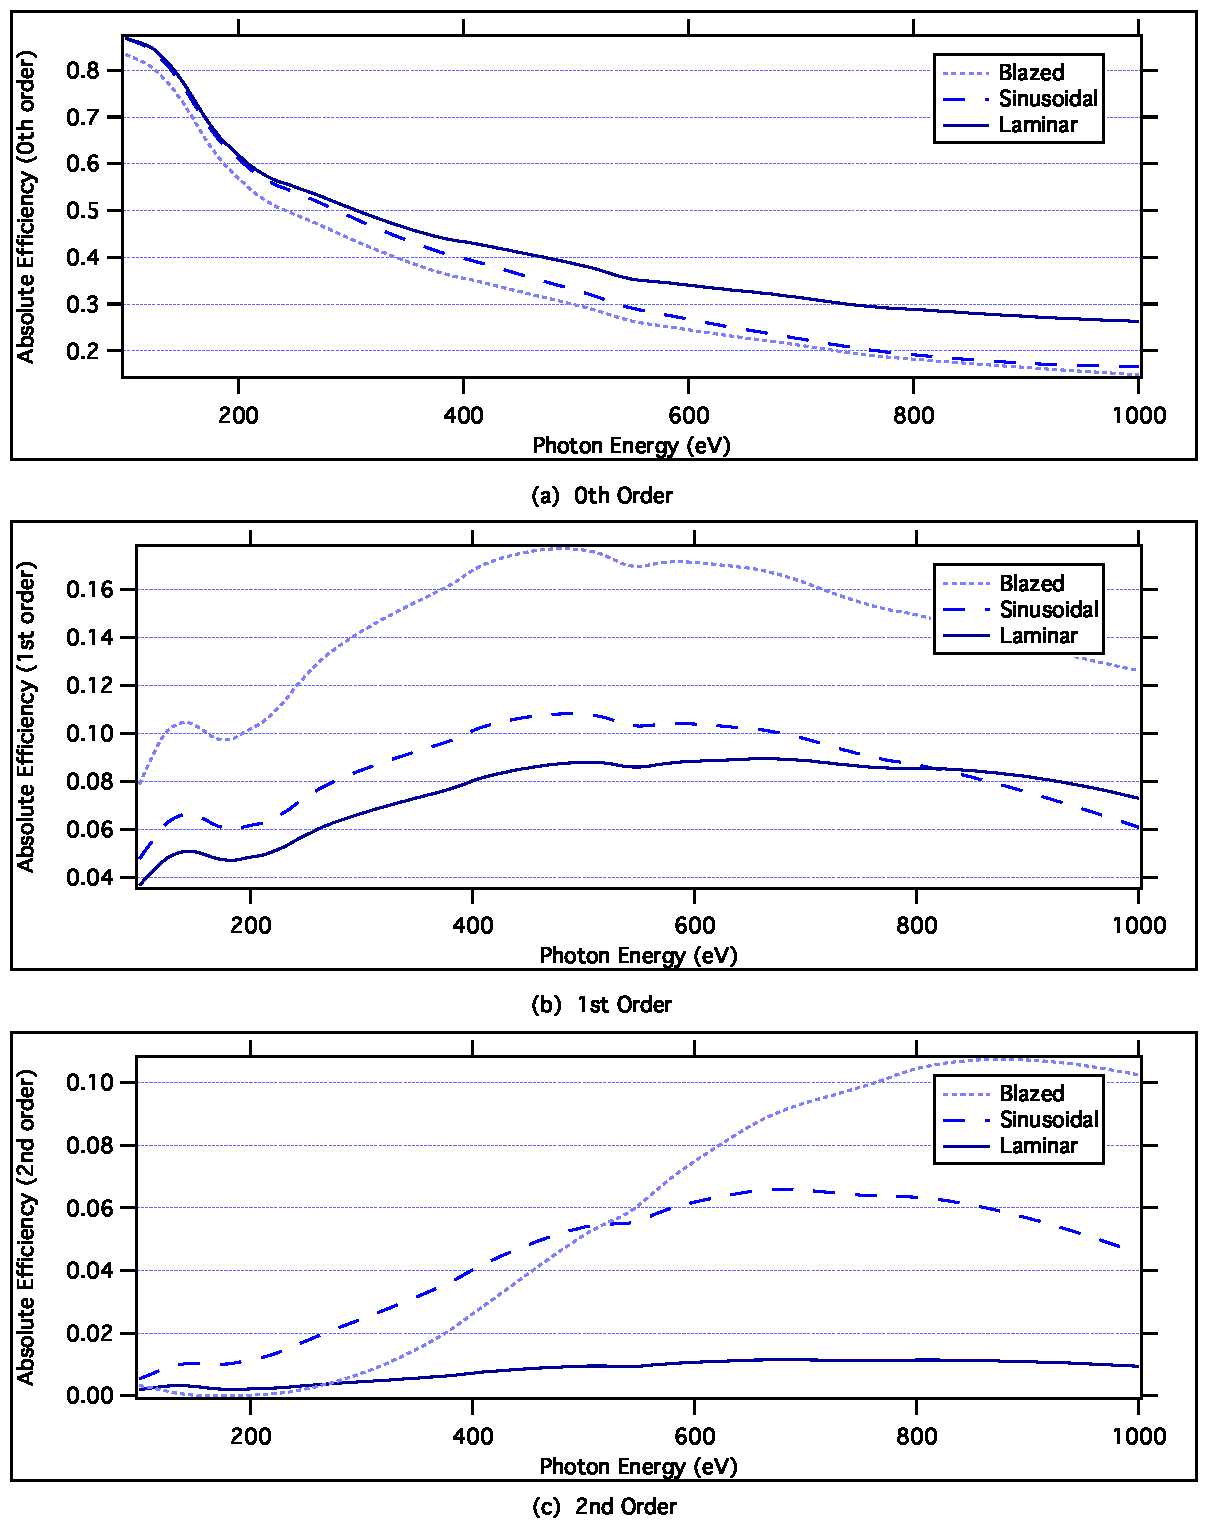
\includegraphics[scale=0.8]{Chapter3/3c_effectOfProfile/3c_3.pdf} 
   \caption{0th order, 1st order, and 2nd order efficiency of three different groove profiles, all optimized for use at 400eV.  The blazed grating is superior in both 1st and 2nd order.  All gratings: 1200 lines/mm, Platinum coating.  Blazed: 1.46$\deg$ angle, 60$\deg$ anti-blaze angle.  Sinusoidal: 13.7nm groove depth.  Laminar (rectangular): 9.6nm groove depth, 50\% duty cycle. }
   \label{3c-plot}
\end{figure}

\subsubsection{Efficiency Comparison of Common Profiles}
For comparison, Figure \ref{3c-plot} shows the 0th order, 1st order, and 2nd order efficiency for three common grating profiles: blazed, sinusoidal, and rectangular (commonly referred to as \emph{laminar}).  All three gratings have a groove density of 1200 lines/mm, are shown at an incidence angle of 88 degrees, and have had their geometry optimized for maximum efficiency in 1st-order with 400eV photons.  (The coating is platinum, and the substrate is quartz [SiO$_2$].)  The blazed grating was optimized by adjusting the blaze angle; the sinusoidal grating by adjusting the groove depth, and the rectangular grating by adjusting the groove depth and assuming a duty cycle of 50\%.

The blazed profile is substantially superior to both the sinusoidal and laminar alternatives.  In first order, even though the efficiency curve peaks near the design energy of 400eV, the performance is better across the entire range from 100eV to 1000eV (and beyond).  The blaze effect causes this curve to be shifted up in energy by a factor of 2 in 2nd order, so that again the blazed grating out-performs the other profiles, but only above 500eV.  The sinusoidal grating has relatively flat efficiency across the energy range, even though it still shows the energy-dependence of its optimization for 400eV.   (We've chosen a platinum coating for these demonstrations since its reflectivity is relatively constant across the energy range; see Figure \ref{3g-2}.  The small universal dip in efficiency at 180eV is due to a drop in the Pt reflectivity here.)

\subsection{Effect of Groove Density}
Because the groove density directly affects the angular dispersion, using a higher-density grating is the most direct path to designing a higher-resolution instrument (Section \ref{resolutionGoals}).  Unfortunately, Figure \ref{3e} shows that increasing the groove density universally decreases the grating efficiency in all orders except the 0th order, even when the remaining parameters are adjusted to keep the grating optimized.  This turns out to be true, not only in this example for two grating profiles, but as a general principle.  Intuitively, we can argue that as the groove density approaches infinite, the grating will look more and more like a flat mirror -- with microstructure becoming smaller and smaller.  Therefore, it makes sense that the amount of light in the 0th-order specular reflection will increase at the expense of the diffracted orders.

Figure \ref{3e-2} explores the groove density effect in more detail, with an efficiency spectrum for a series of blazed gratings from 300 lines/mm to 2700 lines/mm, all optimized for 400eV at 88$\deg$ incidence.  (TODO: Comment on width of blazing peak? Does blazing become less pronounced at higher groove densities?)

TODO generate 3e-2. (3e-2.xls for data)
	
\begin{figure}[htbp] %  figure placement: here, top, bottom, or page
   \centering
   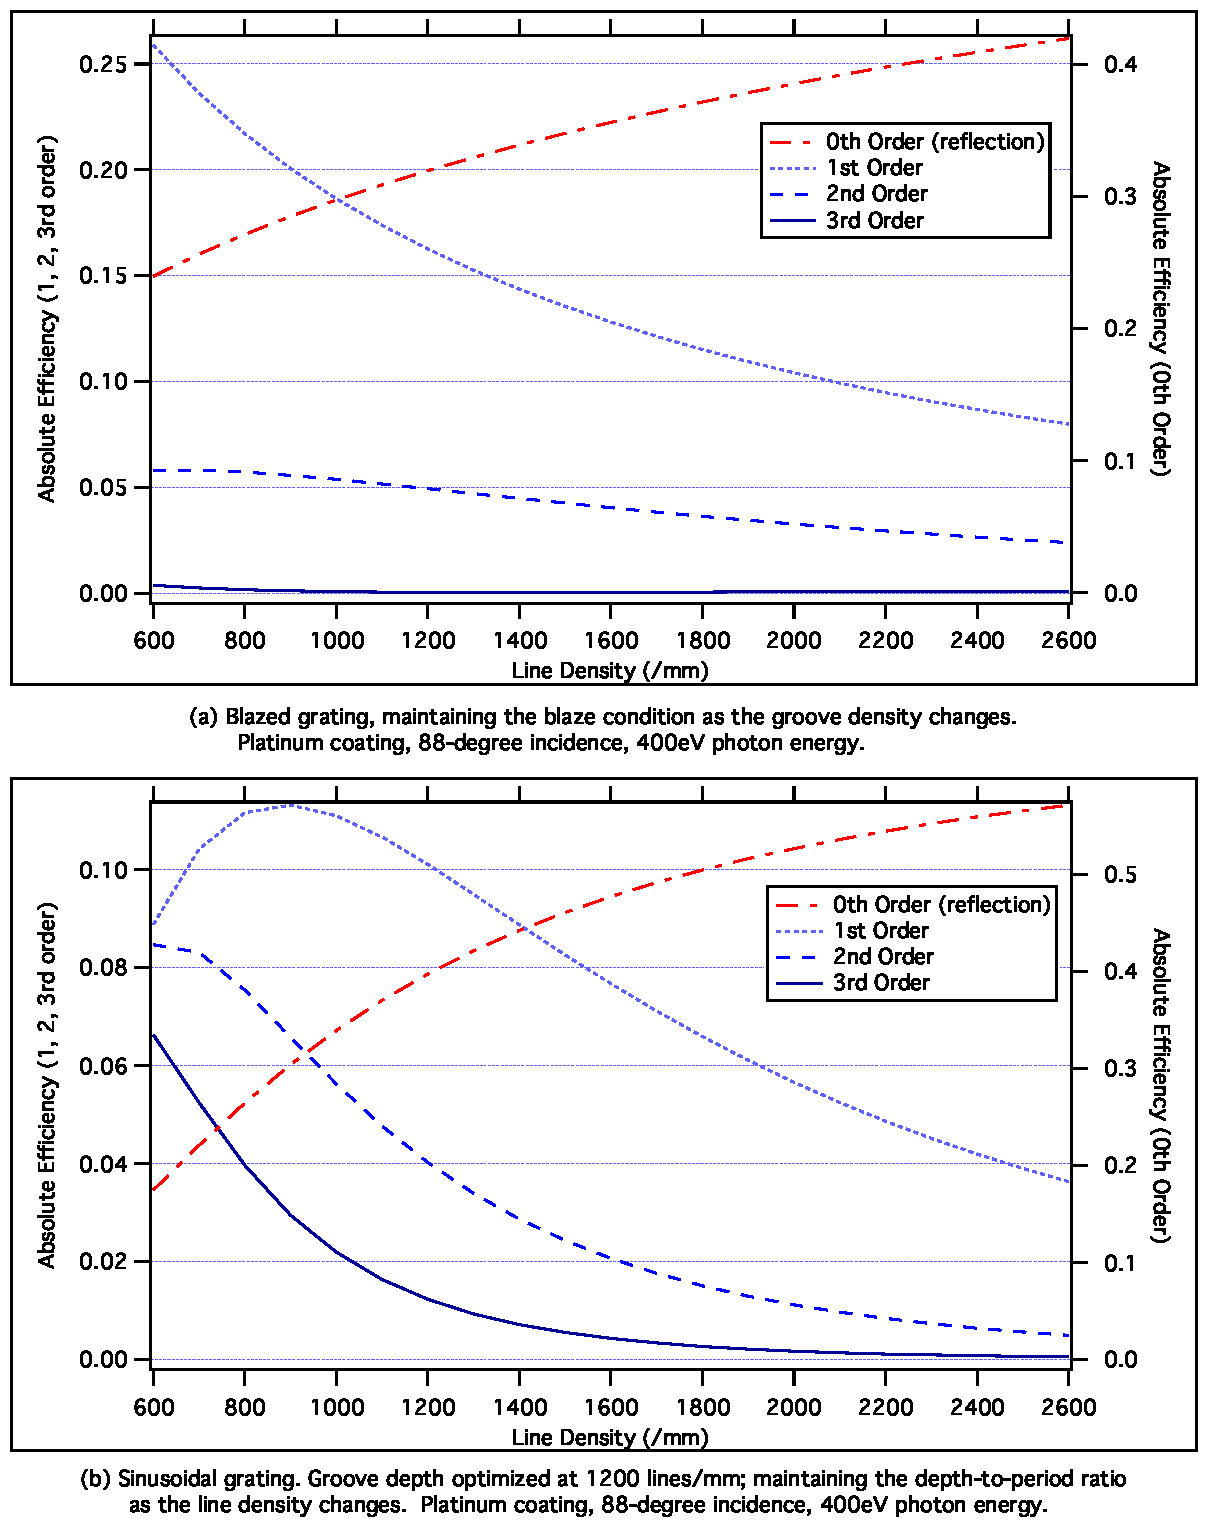
\includegraphics[scale=0.8]{Chapter3/3e_effectOfGrooveDensity/3e.pdf} 
   \caption{Increasing the groove density always decreases the diffraction efficiency -- at least for all the useful orders ($n \neq 0$).  In these plots, we've tried to control for inter-related factors: For the blazed grating in (a), the blaze angle has been adjusted with the groove density (using Equation \ref{blazeAngleEqn}) to maintain the on-blaze condition.  In (b), the sinusoidal grating depth was optimized at 1200 lines/mm, and then the depth-to-period ratio was maintained across changes to the groove density.}
   \label{3e}
\end{figure}

\subsection{Effect of Coating Thickness}
Gratings intended for use in soft x-ray instruments are manufactured on precision-ground  blanks, usually consisting of fused quartz (SiO2) or other amorphous glasses.  The insulating (dielectric) blank is coated in a layer of metal, where the smoothness of the surface is absolutely critical.  Often gold is used as a first coating, since it can be applied with very low roughness, and because it provides a soft layer in which to rule the grooves.  If another type of coating is required (such as nickel and platinum, in our case), these coatings are applied on top of the gold after ruling.

The required thickness of the coating is another question that can be answered by efficiency calculations.   Thin coatings can be applied more smoothly than thick ones (TODO ref Gratings Slits and Mirrors), so the question is: how thick must a coating be for a given photon energy and incidence angle, so that photons are fully reflected or absorbed before reaching the substrate interface?  If the coating is too thin, the absorption characteristics of the glass oxide substrate will start to show up in the efficiency spectrum.

\begin{figure}[htbp] %  figure placement: here, top, bottom, or page
   \centering
   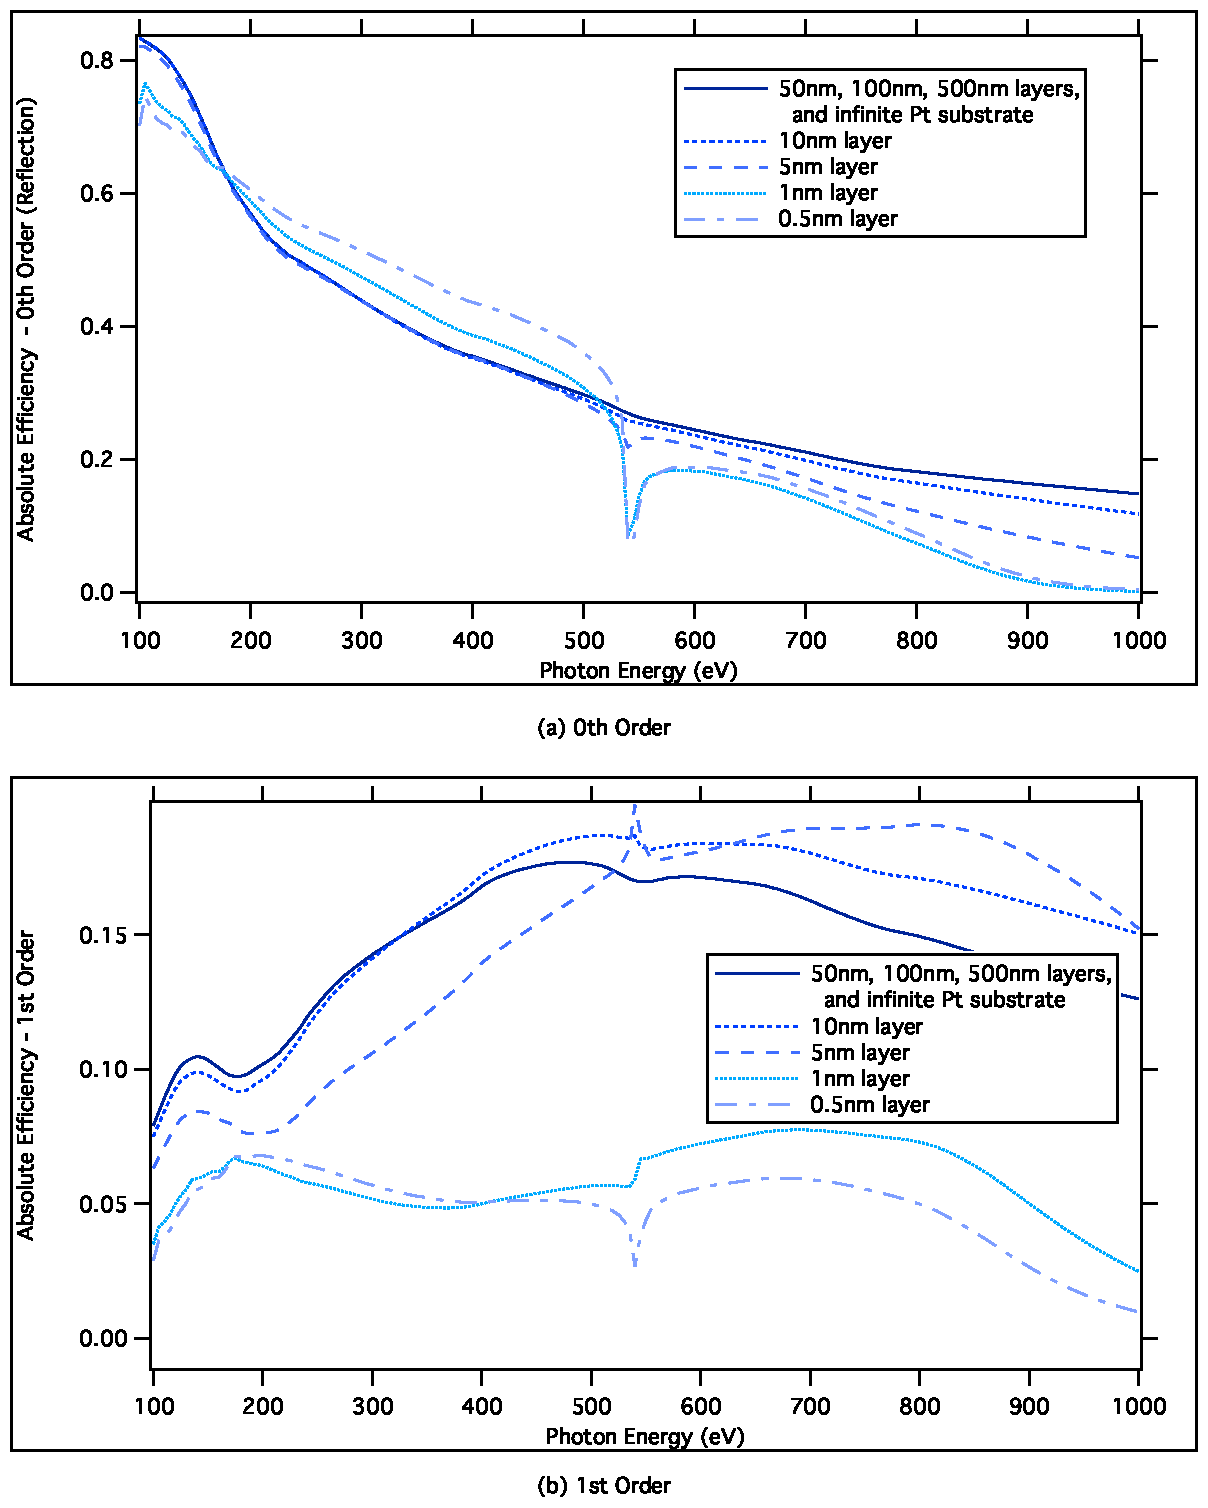
\includegraphics[scale=0.8]{Chapter3/3f_coatingThickness/3f.pdf} 
   \caption{In the soft x-ray regime under grazing incidence, metal-coated dielectric gratings are indistinguishable from pure metal gratings\ldots as long as the coating is thicker than $\sim$ 20nm (although the exact thickness depends on the material, photon energy, and incidence angle).  These calculations show Pt coatings of varying thickness over an SiO$_2$ substrate, as well as an infinitely thick pure Pt grating.  (Blazed grating, 1200 lines/mm, 1.46$\deg$ blaze angle, 88$\deg$ incidence.}
   \label{3f}
\end{figure}

Figure \ref{3f} shows calculations for various thicknesses of platinum coatings above an SiO$_2$ substrate, compared with a theoretical solid platinum grating of infinite thickness.  The 0.5nm and 1nm coatings show the oxygen absorption edge at 525eV, as well as significantly reduced reflectivity over the whole energy range.  The 5nm layer shows a thin-film interference effect that actually boosts the efficiency above 600eV.\footnote{The sharp peak in this spectrum at 525eV might be anomalous; the Henke data -- from which we derive the complex refractive index for all these materials -- is admittedly not accurate in the immediate vicinity of absorption edges.}  As we should expect, at a thickness of 50nm and above, the coated gratings become indistinguishable from an infinitely-thick platinum substrate.  

In general, the required minimum thickness will depend on the photon energy, incidence angle, and the x-ray form factor of the coating material -- all of which affect the x-ray penetration depth.  These results show that for thin coatings, the efficiency calculations are able to rigorously incorporate the effects of interference and absorption at the interface with the substrate.

\subsection{Comparison of coating materials}
All materials suffer from inherently low reflectivity at soft x-ray energies.  Even when gratings are used at grazing incidence, designers must carefully choose coating materials to maximize efficiency considering the desired wavelength range of the instrument.  (This becomes particularly frustrating when a material with otherwise high reflectivity has an absorption edge right in the middle of the region of interest.)

To help in selecting materials, Figures \ref{3g} and \ref{3g-2} show several possibly grating coatings: carbon, nickel, gold, platinum, and iridium.  (Figure \ref{3g} shows the reflectivity of a plain mirror made out of these materials over the energy range from 100 to  1000eV, at 88$\deg$ grazing incidence.  Figure \ref{3g-2} compares the mirror reflectivity with the 0th order and 1st order efficiency of a sinusoidal grating, which had its groove depth optimized for 400eV.)

\begin{figure}[htbp] %  figure placement: here, top, bottom, or page
   \centering
   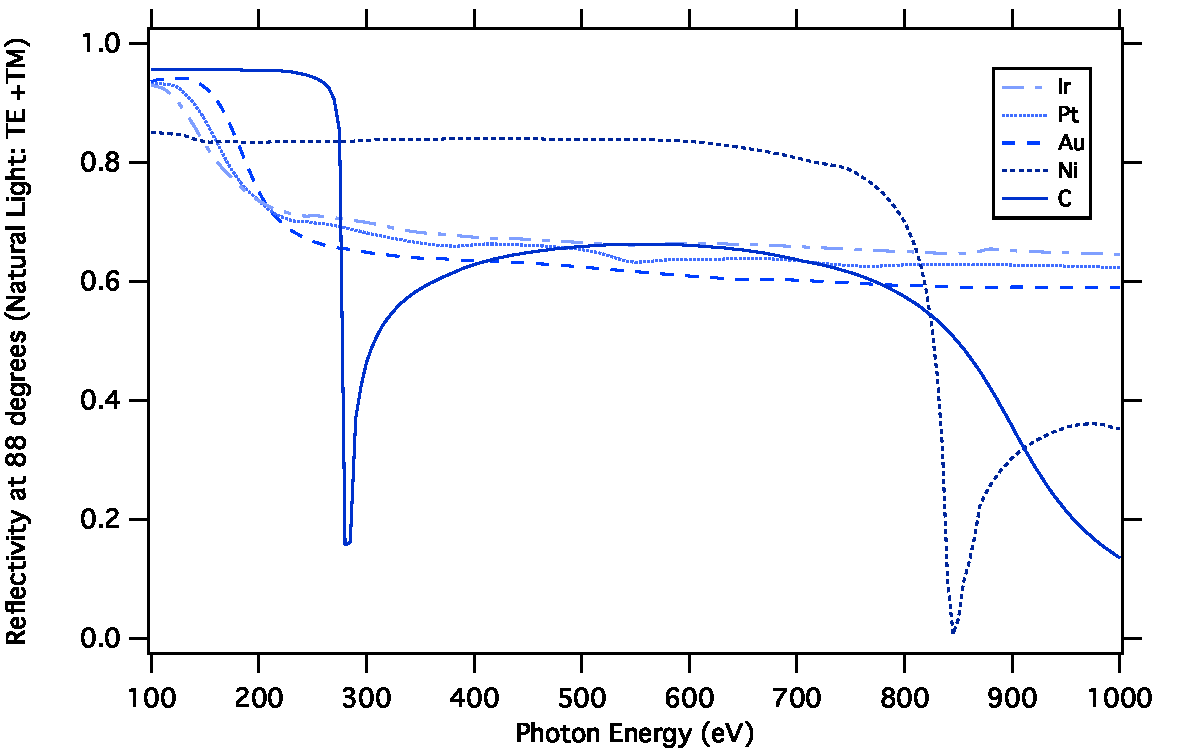
\includegraphics[scale=0.8]{Chapter3/3g_coatingMaterial/3g_reflectivity.pdf} 
   \caption{The reflectivity of a pure mirror at grazing incidence (88$\deg$), as a function of photon energy.  Lighter elements like carbon and nickel have the highest peak reflectivity, but have strong absorption features.  Heavier metals, particularly those within the platinum group, have reasonable reflectivity over the entire soft x-ray region of interest.  Up to 200eV, Gold has a higher reflectivity than Pt and Ir. }
   \label{3g}
\end{figure}

\begin{figure}[htbp] %  figure placement: here, top, bottom, or page
   \centering
   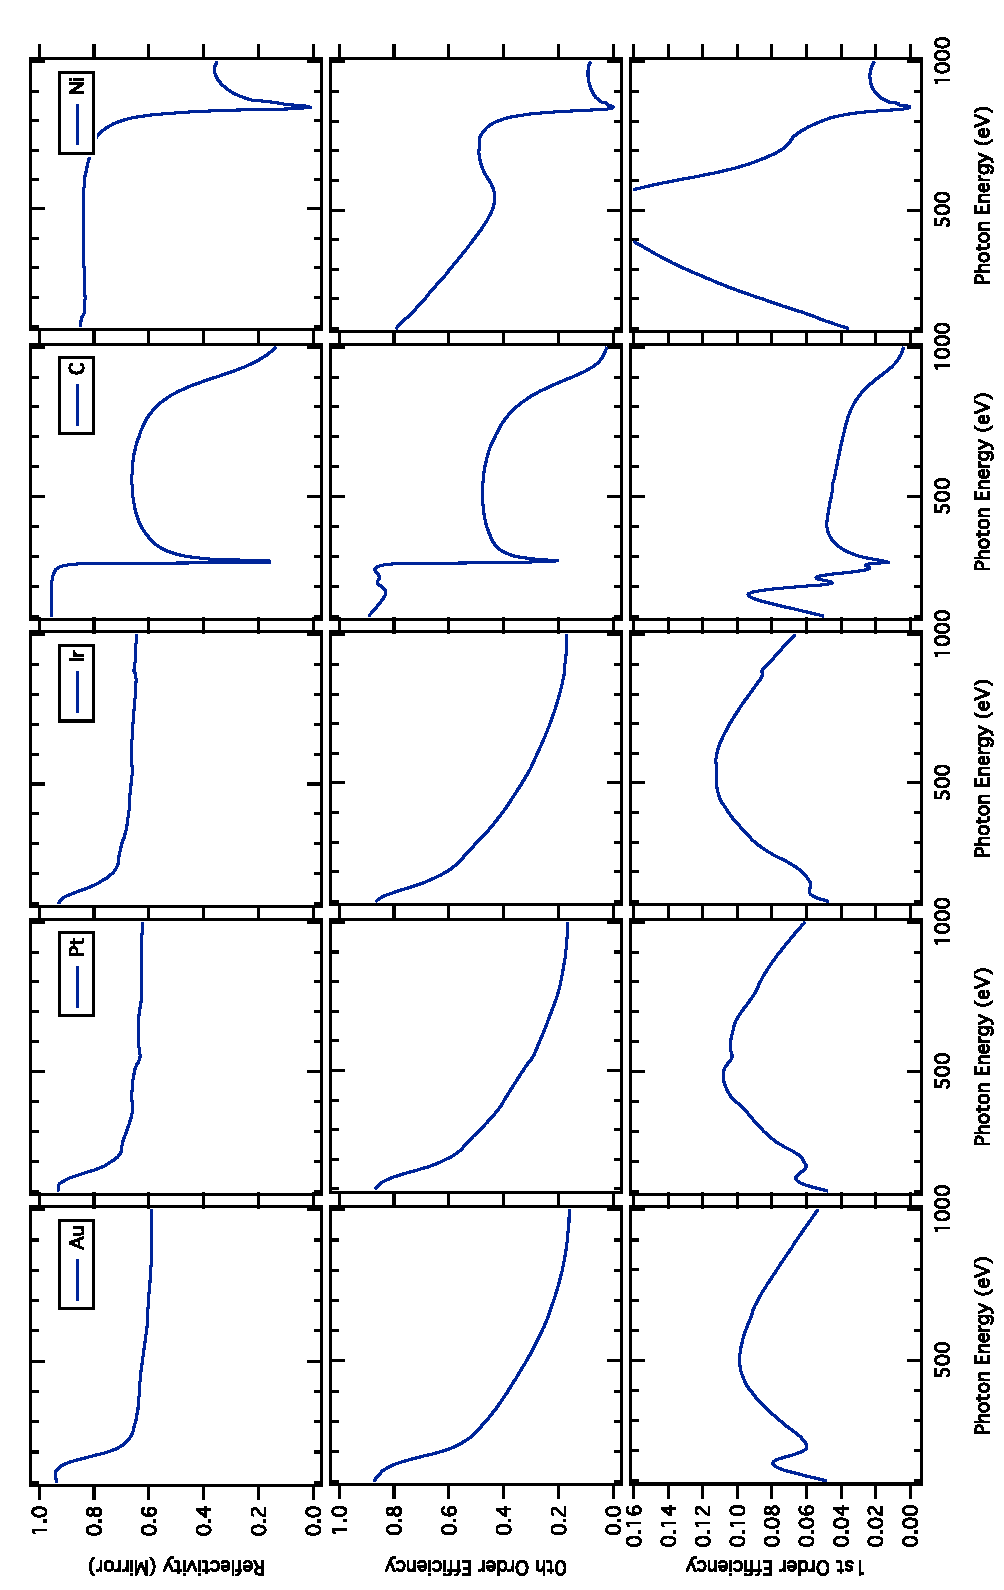
\includegraphics[scale=0.8]{Chapter3/3g_coatingMaterial/3g_multiview.pdf} 
   \caption{A comparison of the mirror reflectivity, 0th order, and 1st order efficiency for different coating materials, as a function of photon energy.  (Gratings: Sinusoidal profile, 88$\deg$ incidence angle, 1200 lines/mm, 13.7nm groove depth)  Note that the 1st order efficiency has energy-dependent features that aren't visible in the simple reflectivity.}
   \label{3g-2}
\end{figure}

The heavy precious metals (Au, Pt, Ir) are commonly chosen for grating coatings because they have a relatively constant reflectivity over this energy range.  This is because their core-level electrons are so tightly bound that their strongest absorption features occur well above the soft x-ray range.  (For example, the Pt K~1s absorption edge is at 78.4 keV.)  Their outer-shell electrons fall within the soft x-ray range (for example, the platinum N and O transitions), but these absorption features aren't nearly as strong, and therefore don't seriously affect the reflectivity.  Gold has better reflectivity than Pt and Ir below 200eV, and also has the previously-mentioned desirable property of being easy to apply smoothly and rule mechanically.  Above 200eV, platinum has been the de-facto choice for high-energy wide-bandwidth gratings for many years.  Iridium (and rhodium, not shown) actually have even better reflectivity and corrosion resistance than platinum, and are becoming standard coating options with some manufacturers.

In contrast, carbon and nickel offer much higher reflectivity over some parts of this energy range, but unfortunately have strong absorption features right in the middle.  The carbon K 1s absorption edge at 284eV makes it restricted to, but excellent for, low-energy applications.  The nickel L$_2$/L$_3$ edges don't occur until 870/853 eV, and Figure \ref{3g-2} seems to suggest that nickel would be the clear winner over much of the soft x-ray range.  This prompted us to use it for two of the REIXS spectrometer gratings, with one obvious but unforeseen consequence (Section \ref{nickelOxidation}).

Not shown in these plots, silicon also has a very high reflectivity up to its L$_2$/L$_3$ absorption edge at 100eV. Therefore, bare (uncoated) SiO$_2$ mirrors are often used for extreme ultra-violet (EUV) and very low-energy soft x-ray beamlines (TODO REF Gratings, Slits and Mirrors); Si-coated gratings might be useful here as well.

\subsection{Effect of photon energy / wavelength}
The energy-dependence (or wavelength-dependence) of grating efficiency has been shown in many of the previous plots, where we've displayed the efficiency as a function of photon energy.  However, it's impossible to completely isolate this relationship because the photon energy is inherently coupled to the grating efficiency in multiple ways.  For starters, the complex refractive indexes of the coating and substrate vary as a function of energy.  However, the photon energy also determines the angle of the outgoing diffraction orders, which can be seen in both the Rayleigh expansion for the total field, and in the simplified grating equation (Equation \ref{gratingEquation}).  Therefore, optimizations for geometry parameters that depend on angle -- like the blaze angle and groove depth -- are inherently coupled to the photon energy.  The plots in Figure \ref{3e-2} highlight this by showing the difference between the energy-dependent reflectivity of a plain flat mirror, versus the more complicated diffraction efficiency.

\subsection{Effect of incidence angle}
In the soft x-ray regime, the real part of the refractive index for most metals is less than unity.  This means that the phase velocity for light in the material is actually \emph{faster} than the speed of light in a vacuum.\footnote{The non-zero imaginary part of the refractive index ensures that the transmitted wave decays and is absorbed, therefore Einstein's speed limit is not violated.}  As mentioned in Section \ref{TER-intro}, we can exploit this lucky phenomenon to increase the reflectivity of gratings and mirrors by using them at grazing incidence to create a \emph{``total external reflection''}.

Total internal reflection (TIR) happens in conventional materials when a light ray travels from a slower optical medium (refractive index $n_1$) toward a faster optical medium (refractive index $n_2 < n_1$).  Snell's law of refraction would relate the angles of the incident ($\theta_1$) and transmitted ($\theta_2$) waves:
\begin{eqnarray}
n_1 \sin \theta_1 &=& n_2 \sin \theta_2 \\
\sin \theta_2 &=& \frac{n_1}{n_2} \sin \theta_1
\end{eqnarray}
By choosing an incident angle $\theta_1$ for which there is no possible solution to $\theta_2$, we can ensure that there is no transmitted wave -- the incident wave must be completely reflected.
\begin{eqnarray}
 \frac{n_1}{n_2} \sin \theta_1 &>& 1
\end{eqnarray}
This will happen for all incident angles $\theta_1$ beyond a critical angle:
\begin{eqnarray}
\theta_{\mathrm{critical}} &=& \arcsin \left( \frac{n_2}{n_1} \right)
\end{eqnarray}

The same situation happens when light from the (slower) vacuum is incident on the (faster) medium of the grating.  Here the vacuum refractive index is $n_1=1$, and the real part of the grating refractive index (which gives the propagation velocity) is $\tilde {n}_2<1$.  (For example, at 410 eV, the real part of the refractive index of gold is $\tilde{n}_2 = 0.99425$.)  We can therefore calculate the critical angle for \emph{total external reflection}; for incident angles larger than this, there should be no transmitted wave into the grating:
\begin{eqnarray}
\theta_{\mathrm{critical}} &=& \arcsin \left( \tilde n \right)
\end{eqnarray}
(where $\tilde n$ is the real part of the coating's complex refractive index.)  Critical angles for the coatings in Figure \ref{3g-2} at 410eV are given in Table \ref{3i-2}.

\begin{table}[htbp]
   \centering
   \caption{Critical incidence angles for ``total external reflection'' at 410 eV for the grating coatings shown in Figure \ref{3g-2}.}
   \begin{tabular}{@{} r c @{}} % Column formatting, @{} suppresses leading/trailing space
      \hline
        Material    & $\theta_{\mathrm{critical}}$ for TER ($\deg$)\\
      \hline \hline
Carbon (C) & 85.92\\
Nickel (Ni) & 83.20\\
Gold (Au)& 83.85\\
Platinum (Pt)& 83.32\\
Iridium (Ir)& 83.10\\
      \hline
   \end{tabular}
   \label{3i-2}
\end{table}

The concept of TER is just another intuitive approximation for what happens in the full electromagnetic picture, but Figure \ref{3i} does confirm that the grating efficiencies in the 0th, 1st, and 2nd inside orders are indeed extremely low below platinum's critical incidence angle of 83.3$\deg$.  This figure shows the effect of incidence angle on efficiency for several different geometry profiles.  We might expect that as the incidence angle becomes more and more grazing, the efficiency should increase continuously\ldots and that is certainly true for the $n=0$ order.  However, this turns out to be not true for the remaining orders; \emph{there is actually an optimal incidence angle below $90\deg$ where efficiency is maximized}.  At first glance, it might seem like this is an accidental side-effect of the blazed optimization; since the optimal blaze angle depends on the incidence angle, it might have been possible that all the gratings in Figure \ref{3j} had their geometry optimized for a sub-$90\deg$ incidence angle.  However, by exploring the effect of incidence angle on efficiency over a range of blaze angles, Figure \ref{3j-2} dispels this idea; it shows that for $n\neq 0$ orders, there is indeed an optimal incidence angle, which depends only on the groove density and the energy.

Figure \ref{3j-2} contains a take-away message for instrument designers: if an arbitrary incidence angle is required for some external reason, the blaze angle can be adjusted to optimize for that incidence. However, in the absence of constraints, there does exist a unique optimal incidence angle (and corresponding blaze angle), typically between $87\deg$ and $88\deg$, where the efficiency reaches an absolute maximum.


\begin{figure}[htbp] %  figure placement: here, top, bottom, or page
   \centering
   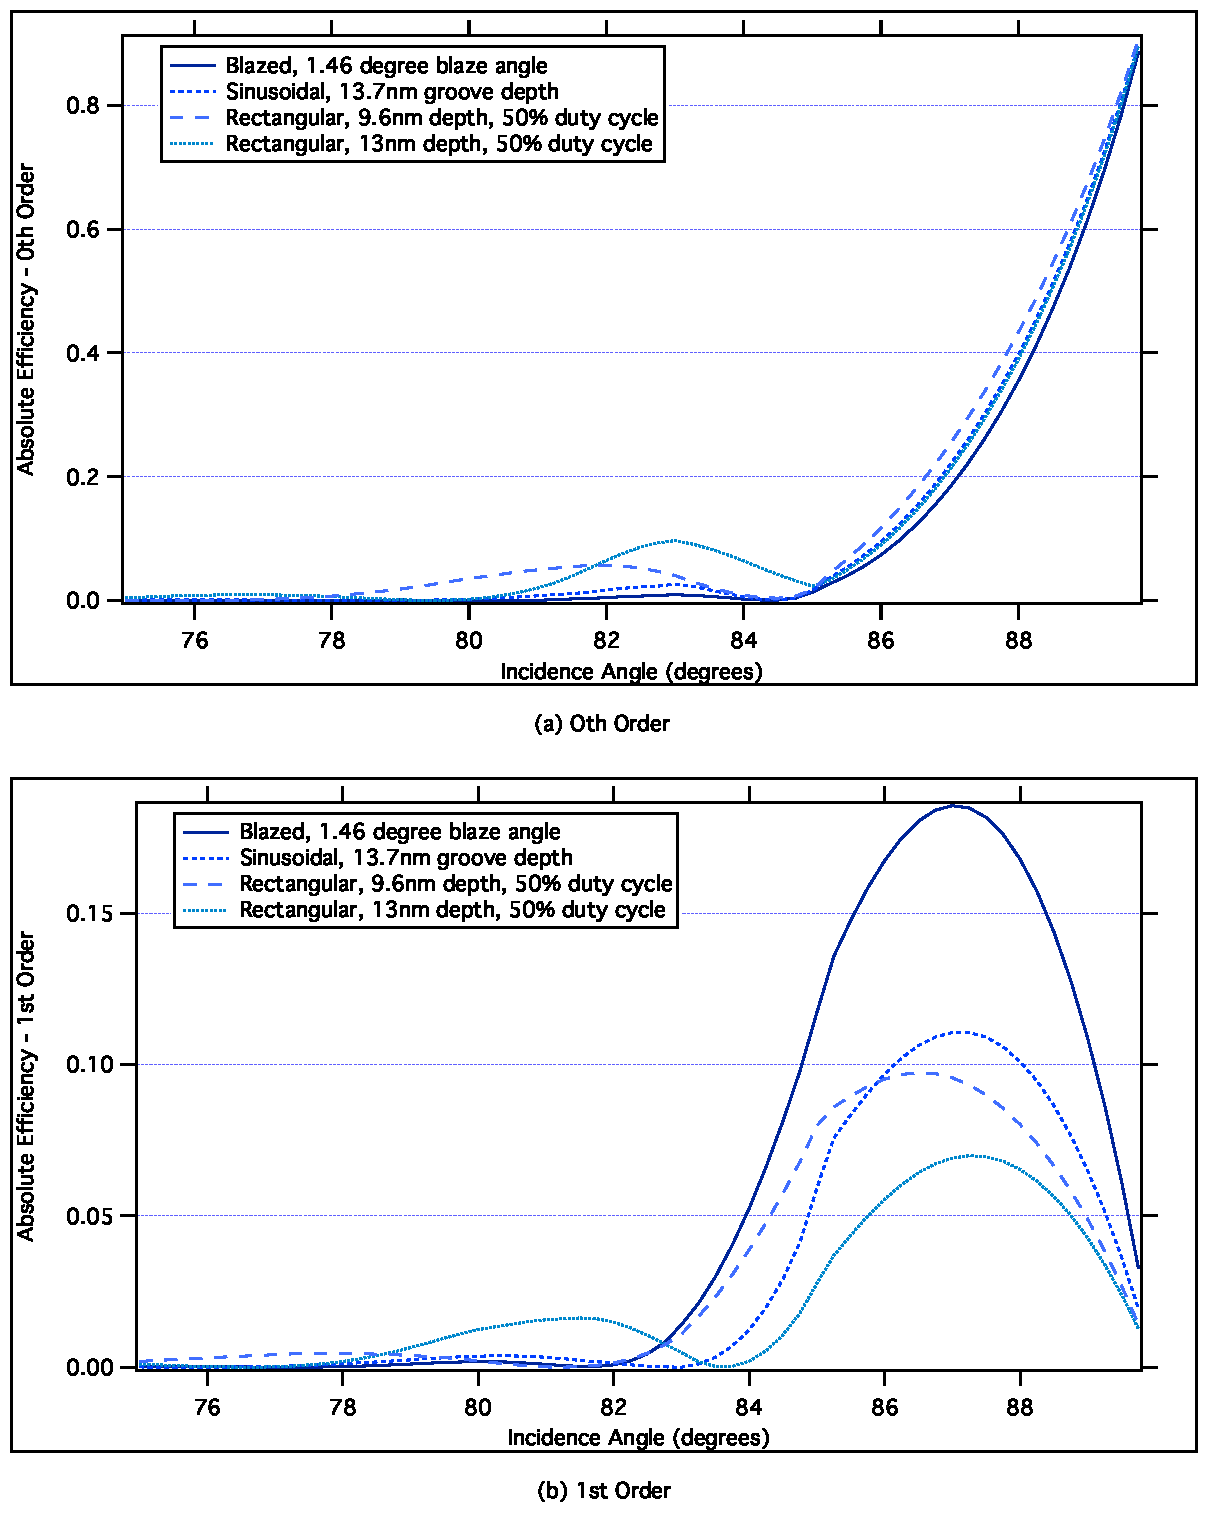
\includegraphics[scale=0.8]{Chapter3/3i_incidenceAngle/3i_variousGratings.pdf} 
   \caption{The effect of incidence angle on diffraction efficiency for various grating profiles.  While the 0th order efficiency/reflectivity always increases as the incident light becomes more grazing, there is an optimal incidence angle below 90$\deg$ for higher-order light.  The critical angle for total external reflection in Platinum is 83.3$\deg$; clearly both the 0th-order and 1st-order efficiency drop off significantly below this angle. (Gratings: 1200 lines/mm, platinum coating, 400 eV; blaze angles and profiles as indicated.)}
   \label{3i}
\end{figure}
	
\begin{figure}[htbp] %  figure placement: here, top, bottom, or page
   \centering
   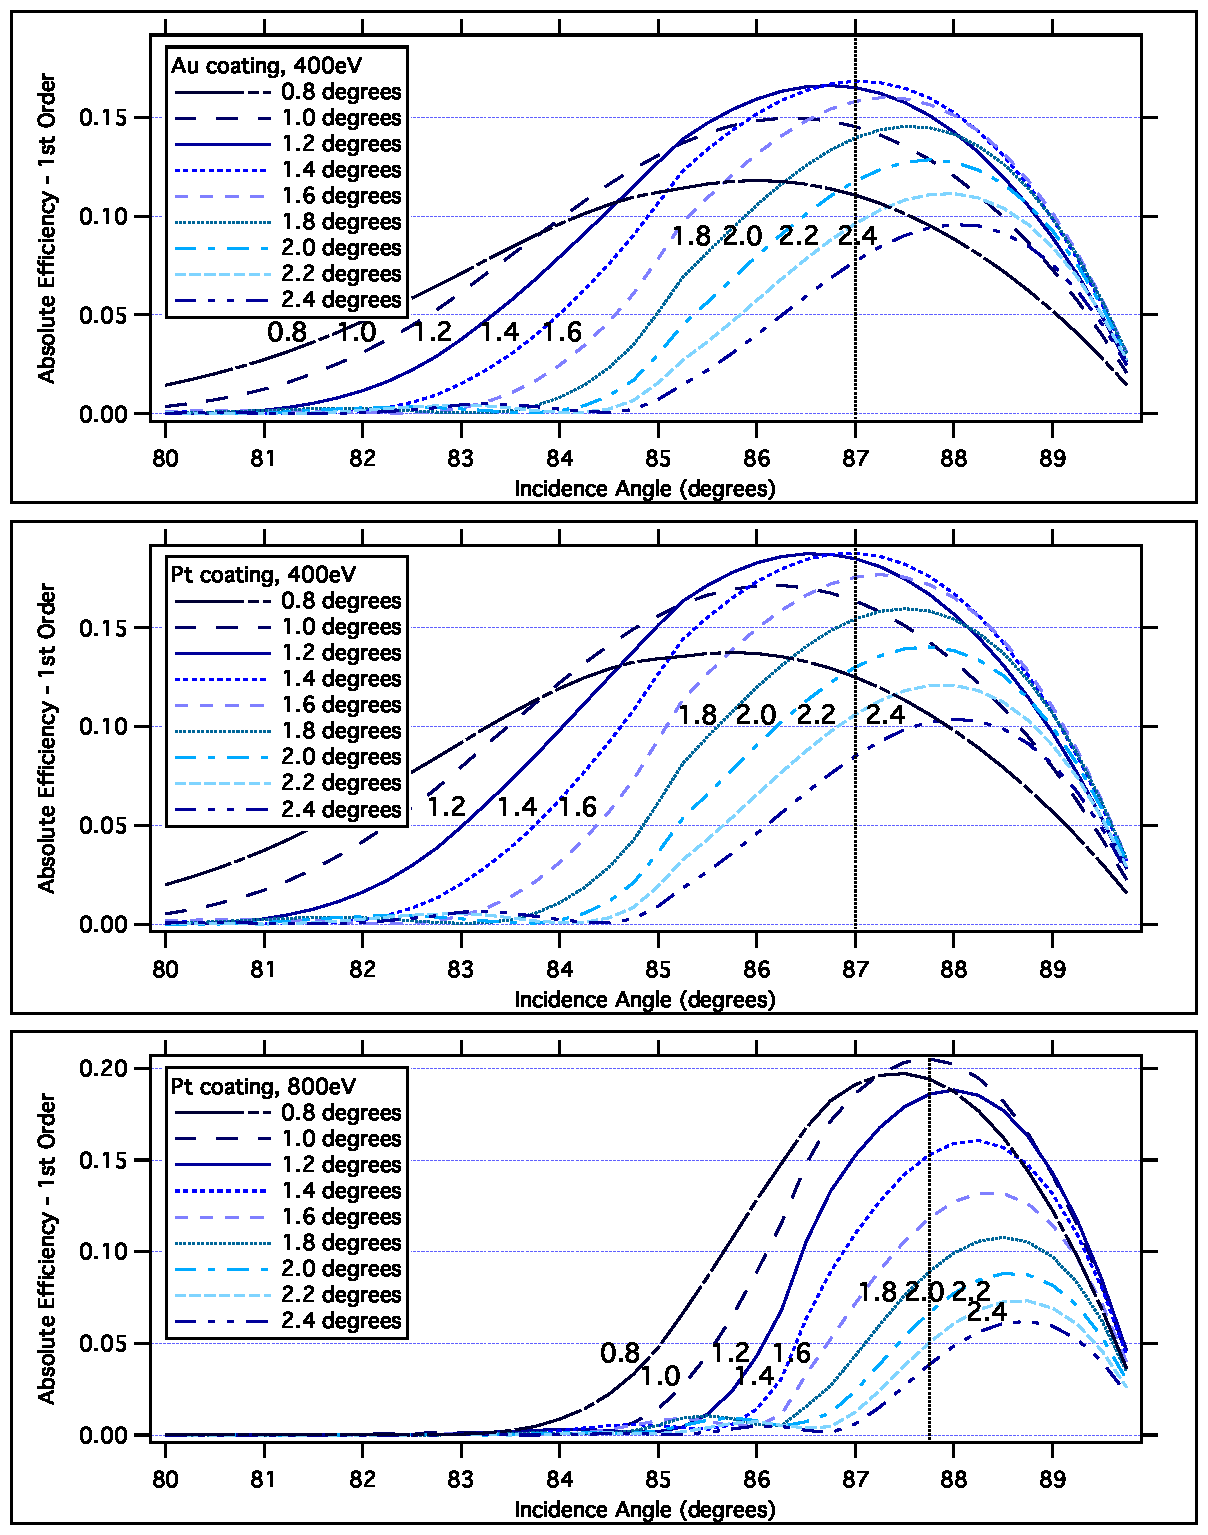
\includegraphics[scale=0.8]{Chapter3/3i_incidenceAngle/3i_blazeChanges2.pdf} 
   \caption{While the blaze angle can always be used to tune a grating for a required incidence angle, there is still a particular \emph{optimal} incidence angle that -- when combined with a corresponding optimized blaze angle -- would produce the highest achievable efficiency.  This optimal angle doesn't seem to depend on the material, but only on the groove density and energy.  (Gratings: all 1200 lines/mm; coatings, blaze angles, and energies as indicated.)}
   \label{3i-2}
\end{figure}

TODO: test with groove density. Does it depend on difffraction eqn?
	
\subsection{TODO Applications to beamline and instrument design}
	- Observation: blaze angle and groove depth can be used to optimize efficiency for a constrained incidence angle.  However, while 0-order reflectivity increases with grazing incidence, there IS an optimal incidence angle (usually between 87 and 88 degrees), which does not depend on the grating material, and depends somewhat on the incident energy (increases with energy).  
	
	Practical application: This optimal incidence angle provided the starting point for the incidence angles used in the REIXS spectrometer, and explains why the lower-energy gratings (LEG, IMP) use lower (more normal) incidence angles than the high-energy gratings.
	TODO if time: determine way to calculate optimal incidence angle.  Is this just a TE or TM effect? NO... te and tm behave the same.
	
	
Highlighted conclusions:
	- blazed is idea for narrow energy range and constant incidence angle.  In case of spectrometer, definitely the right choice.  For mono... No constant incidence angle.  Still better than sinusoidal if not?  Find out.
	
\begin{itemize}
\item Optimal incidence angle
\item always blazed: (show whether better than sinusoidal for CII monochromator)
\item consider 3rd order rather than increasing groove density (manuf. limit) --> next chapter.
\item blazed gratings: when optimizing for low energies (near 100eV): create narrow efficiency peaks. when optimized for higher energies, the peaks are wider and the gratings can be more general.
\end{itemize}

\section{Validation: comparison of theory to experimental results}
The previous section provides some recommendations to beamline designers based on this theoretical survey of the factors affecting grating efficiency.  For these results to be trustworthy, we need confirmation that the theoretical methods in Chapter 3 -- and the software implementation described in this chapter -- accurately describe gratings in the real world.  We go onward in Chapter 5 to use these tools to design the gratings and optical layout for the REIXS beamline spectrometer; before starting this project, we clearly needed our own validation of the software's accuracy.

The published literature on grating efficiency does not contain many measurements of real-world grating efficiency, partly due to the difficulty of completing these measurements, and partly because -- on receiving brand new gratings -- most beamline builders would rather install them as quickly as possible and start doing their own science, rather than spend time on another beamline characterizing the gratings.  We were able to find one study by M. Bowler at the SRS light source (TODO REF Bowler) with a recent set of efficiency measurements done on four gratings, representing three different types of grating profiles, which turned out to be ideal for comparing with theoretical calculations.  The gratings consisted of one blazed grating with 1440 lines/mm, one laminar grating with 600 lines/mm, and two attempted-laminar gratings that ended up with trapezoidal sides of approximately $57\deg$.  All of the gratings were well-characterized by the manufacturer after ruling, allowing for accurate geometry inputs into the theoretical calculations.  (The study also conducted efficiency calculations  using the differential method, but we duplicated these calculations as a double-check on our implementation.)

Figures \ref{3j-1} through \ref{3j-4} show the experimental measurements from (TODO REF), combined with our own calculations of the grating efficiency.  Table \ref{3j-table} provides the geometry parameters, derived from the manufacturer's measurements.

\subsubsection{Note on incidence angle}
Unlike the constant incidence angle efficiency curves we've been using up to this point, these gratings were designed for use in constant-included-angle monochromators, where the deviation angle $(\theta_2 + \theta_{2,n})$ between the incident beam and the useful order $n$ is held constant.  Therefore, these plots show the efficiency as a function of energy, with an incidence angle that also varies according to this constraint as a function of energy along the $x$-axis.

Of particular interest are the 1st and 2nd order results for the blazed grating in Figure \ref{3j-1}, since we settled on blazed gratings for the design in Chapter 5.  The agreement in the shape and amplitude of the efficiency spectra is very good; we can expect that the real-world efficiency would be slightly lower than predicted due to surface roughness and other effects described in Section \ref{realWorldEffects}.  The agreement for the laminar profile in Figure \ref{3j-2} is also very good.  Figures \ref{3j-3} and \ref{3j-4} show a tendency for the calculated results on the trapezoidal gratings to be shifted toward lower energies with respect to the measurements, although the shift is less than 20 eV.  Overall, the close agreement between theoretical and measured efficiencies shown here gives us a high degree of confidence in applying the grating software to optimize real-world beamlines.
 
\begin{figure}[htbp] %  figure placement: here, top, bottom, or page
   \centering
   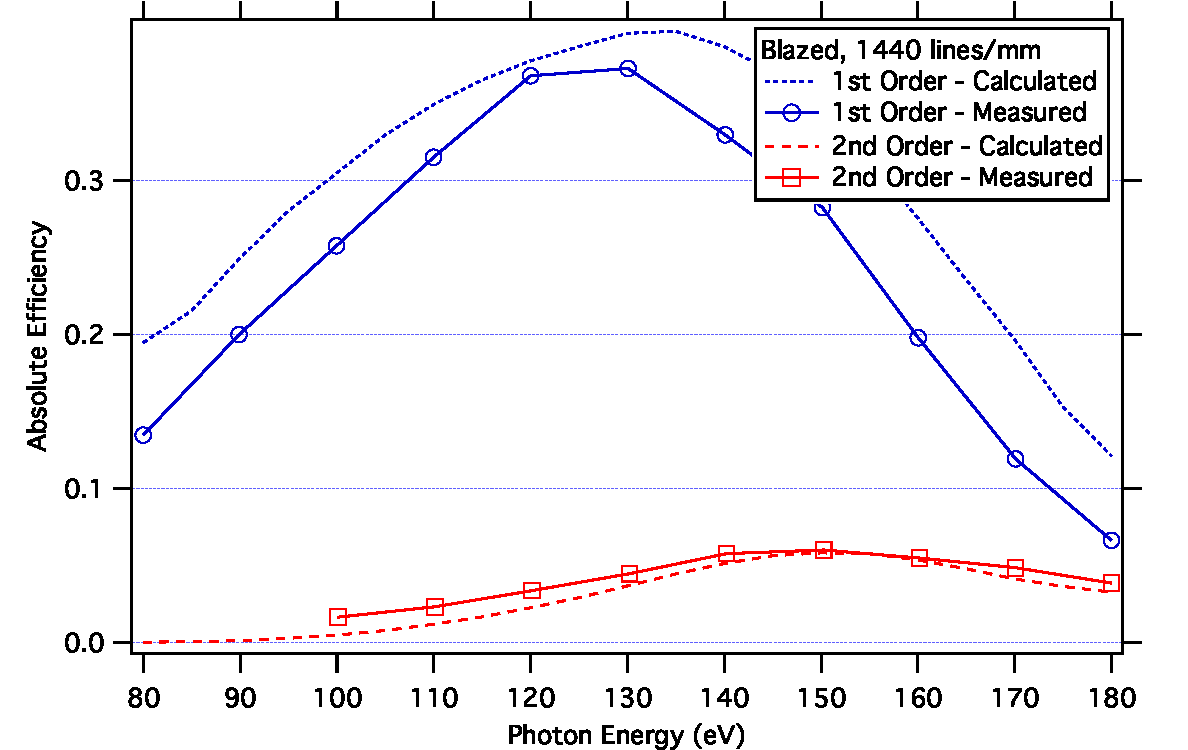
\includegraphics[scale=0.8]{Chapter3/3j_comparisonWithExperimental/3j_blazed.pdf} 
   \caption{Comparison of grating efficiency calculations to diffractometer measurements.  Blazed grating, 1440 lines/mm, 2.2$\deg$ blaze angle, 12.8$\deg$ anti-blaze angle. Incidence: 160$\deg$ constant included angle to the 1st inside order.}
   \label{3j-1}
\end{figure}

\begin{figure}[htbp] %  figure placement: here, top, bottom, or page
   \centering
   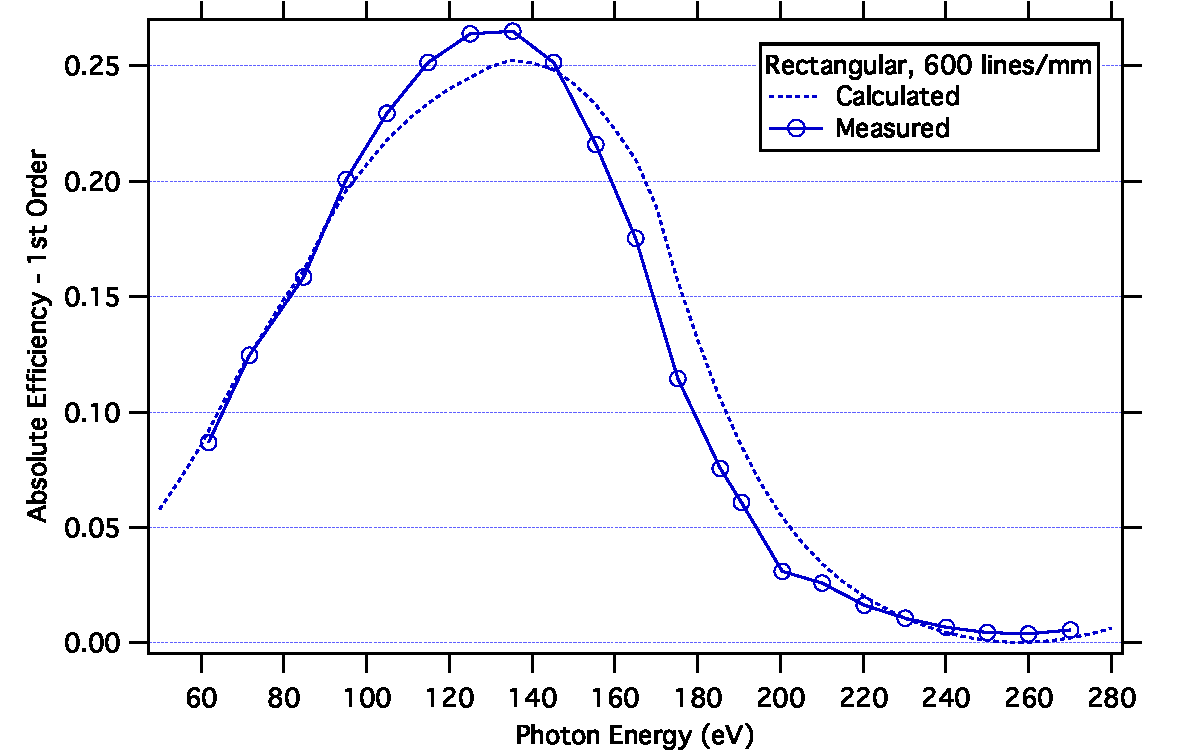
\includegraphics[scale=0.8]{Chapter3/3j_comparisonWithExperimental/3j_laminar.pdf} 
   \caption{Comparison of grating efficiency calculations to diffractometer measurements.  Rectangular grating, 600 lines/mm, 22.2 nm depth, 0.833 um valley width.  Incidence: 167$\deg$ constant included angle to the 1st inside order.}
   \label{3j-2}
\end{figure}

\begin{figure}[htbp] %  figure placement: here, top, bottom, or page
   \centering
   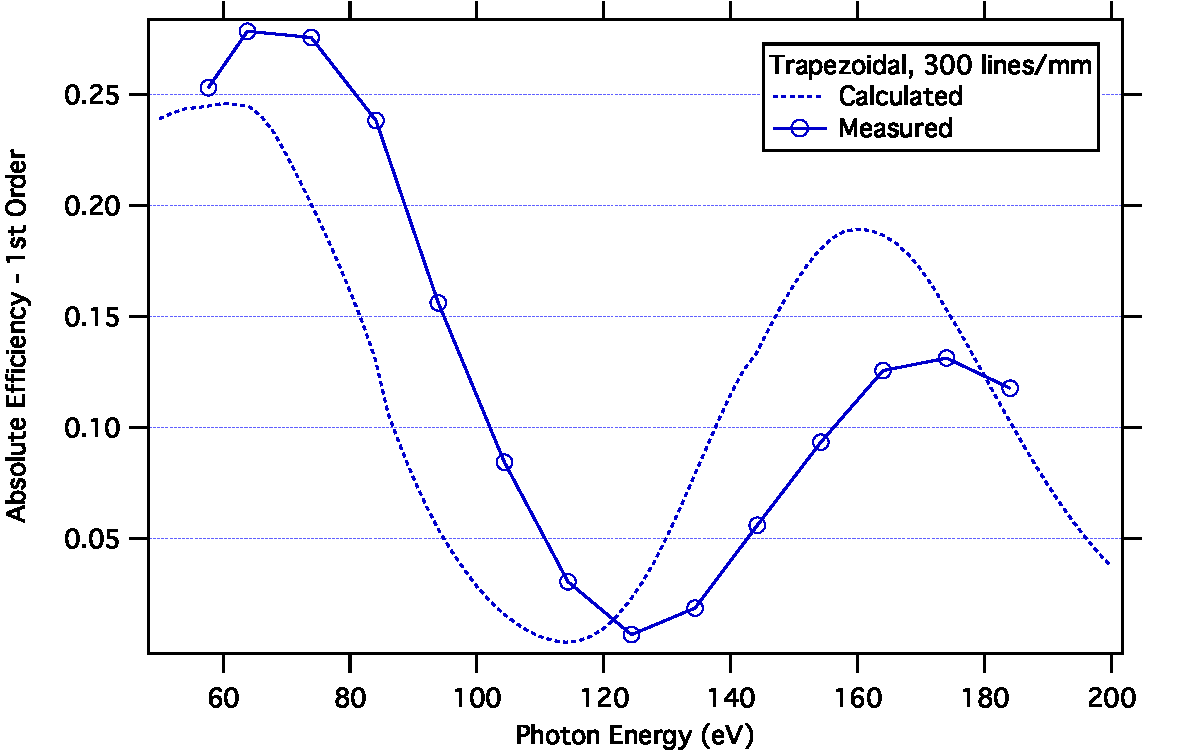
\includegraphics[scale=0.8]{Chapter3/3j_comparisonWithExperimental/3j_trap300.pdf} 
   \caption{Comparison of grating efficiency calculations to diffractometer measurements.  Trapezoidal grating, 300 lines/mm, 57$\deg$ side angles, 49.3 nm depth, 2.46 um valley width.  Incidence: 167$\deg$ constant included angle to the 1st inside order.}
   \label{3j-3}
\end{figure}

\begin{figure}[htbp] %  figure placement: here, top, bottom, or page
   \centering
   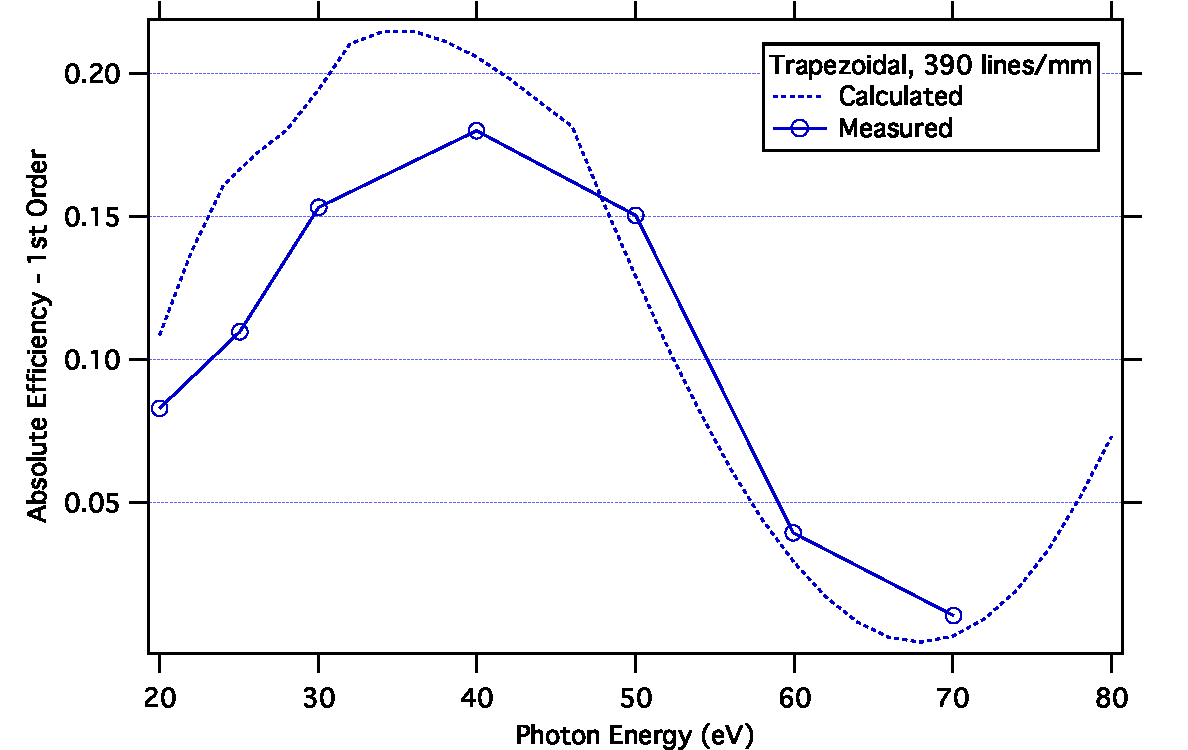
\includegraphics[scale=0.8]{Chapter3/3j_comparisonWithExperimental/3j_trap390.pdf} 
   \caption{Comparison of grating efficiency calculations to diffractometer measurements.  Trapezoidal grating, 390 lines/mm, 57$\deg$ side angles, 54 nm depth, 1.39 um valley width.  Incidence: 160$\deg$ constant included angle to the 1st inside order.}
   \label{3j-4}
\end{figure}
